\documentclass[11pt]{article}
\usepackage[T1]{fontenc}
\usepackage{lmodern}
\usepackage[margin=1in]{geometry}
\usepackage{amsmath,amssymb,amsthm,mathtools}
\usepackage{microtype}
\usepackage{enumerate,booktabs,array}
\usepackage{tikz}
\usetikzlibrary{arrows.meta,calc,decorations.pathreplacing,decorations.markings,positioning,patterns}
\usepackage{xcolor}
\usepackage{hyperref}
\hypersetup{colorlinks=true,linkcolor=blue!45!black,citecolor=blue!45!black,urlcolor=blue!45!black,
  pdftitle={Modularity of elliptic curves over imaginary quadratic fields},pdfauthor={OpenAI}}
\setlength{\emergencystretch}{2em}
\numberwithin{equation}{section}
\newtheorem{theorem}{Theorem}[section]
\newtheorem{proposition}[theorem]{Proposition}
\newtheorem{lemma}[theorem]{Lemma}
\newtheorem{corollary}[theorem]{Corollary}
\theoremstyle{definition}
\newtheorem{definition}[theorem]{Definition}
\newtheorem{remark}[theorem]{Remark}
\newtheorem{example}[theorem]{Example}
\newcommand{\Q}{\mathbb Q}
\newcommand{\Z}{\mathbb Z}
\newcommand{\C}{\mathbb C}
\newcommand{\R}{\mathbb R}
\newcommand{\F}{\mathbb F}
\newcommand{\A}{\mathbb A}
\newcommand{\Gm}{\mathbb G_m}
\newcommand{\Qbar}{\overline{\Q}}
\newcommand{\eps}{\epsilon}
\DeclareMathOperator{\GL}{GL}
\DeclareMathOperator{\SL}{SL}
\DeclareMathOperator{\PGL}{PGL}
\DeclareMathOperator{\Gal}{Gal}
\DeclareMathOperator{\Spec}{Spec}
\DeclareMathOperator{\Res}{Res}
\DeclareMathOperator{\Jac}{Jac}
\DeclareMathOperator{\Pic}{Pic}
\DeclareMathOperator{\Hom}{Hom}
\DeclareMathOperator{\End}{End}
\DeclareMathOperator{\Aut}{Aut}
\DeclareMathOperator{\Tr}{Tr}
\DeclareMathOperator{\tr}{tr}
\DeclareMathOperator{\im}{im}
\DeclareMathOperator{\id}{id}
\DeclareMathOperator{\diag}{diag}
\DeclareMathOperator{\HT}{HT}
\DeclareMathOperator{\WD}{WD}
\DeclareMathOperator{\rec}{rec}
\DeclareMathOperator{\Frob}{Frob}
\newcommand{\et}{\mathrm{\acute et}}
\newcommand{\semisimple}{\mathrm{ss}}
\newcommand{\Fss}{\mathrm{F\text{-}ss}}
\newcommand{\ord}{\mathrm{ord}}
\newcommand{\pst}{\mathrm{pst}}
\newcommand{\cris}{\mathrm{cris}}
\newcommand{\st}{\mathrm{st}}
\newcommand{\cO}{\mathcal O}
\newcommand{\cJ}{\mathcal J}
\newcommand{\cC}{\mathcal C}
\newcommand{\cE}{\mathcal E}
\newcommand{\cV}{\mathcal V}
\newcommand{\cL}{\mathcal L}
\newcommand{\into}{\hookrightarrow}
\newcommand{\surj}{\twoheadrightarrow}
\title{Modularity of elliptic curves over imaginary quadratic fields}
\author{OpenAI}
\date{October 4, 2026}
\begin{document}
\maketitle
\begin{abstract}
We prove the modularity conjecture for elliptic curves over imaginary
quadratic fields: every such curve is modular, with matching local
parameters at every place.
\end{abstract}
\section{Introduction}\label{sec:introduction}

Let $K$ be an imaginary quadratic number field and let $E/K$ be an
elliptic curve. The automorphy conjecture for $E$ asks for an automorphic
representation of $\GL_2(\A_K)$ whose local parameters realize the
cohomology of $E$. At a place of good reduction this requires the Hecke
polynomial to recover the point count of the reduced curve; at a bad
place it requires the full local parameter, including its inertia and
monodromy. At infinity the parameter is prescribed by the Hodge types
$(1,0)$ and $(0,1)$.

We prove this conjecture for every $K$ and $E$. We use unitary
normalization on the automorphic side and the Tate-normalized local
Langlands correspondence on the cohomological side. These conventions
are recalled in Section~\ref{sec:conventions}.

\begin{theorem}\label{thm:main}
Let $K$ be an imaginary quadratic number field and $E/K$ an elliptic
curve. There is an isobaric automorphic representation $\pi_E$ of
$\GL_2(\A_K)$ with trivial central character and weight zero such that,
for every prime $l$ and every isomorphism
$\iota:\overline\Q_l\xrightarrow{\sim}\C$,
\[
 r_\iota(\pi_E)\simeq
 H^1_{\et}(E_{\overline K},\overline\Q_l).
\]
At every finite place $v\nmid l$ one has
\[
 \iota\WD\bigl(H^1_{\et}(E_{\overline K},\overline\Q_l)
                     |_{G_{K_v}}\bigr)^{\Fss}
 \simeq
 \rec_{K_v}\bigl(\pi_{E,v}\otimes|\det|_v^{-1/2}\bigr).
\]
The unitary parameter at the complex place is
$z\mapsto\diag(z/|z|,\overline z/|z|)$.
In particular every local factor agrees, and
\[
 L(E/K,s)=L(\pi_E,s-1/2).
\]
If $E$ has no complex multiplication, $\pi_E$ is cuspidal. In the CM
case it is given by automorphic induction of a Hecke character, or by
an isobaric sum when the CM field is already $K$.
\end{theorem}

Here $r_\iota$ in the CM isobaric case is the sum of the corresponding
character realizations with the same Tate normalization.

\subsection{Historical context}

The arithmetic groups associated with imaginary quadratic fields and
their action on hyperbolic three-space originate in Bianchi's
work~\cite{Bianchi}. Their presentations and cohomology were developed
further by Swan and Harder~\cite{Swan,Harder}. The expected relationship
with elliptic curves belongs to the Langlands program: in
\cite[Section~7]{LanglandsProblems}, Langlands explicitly discusses the
automorphy of local representations attached to elliptic curves over
global fields of characteristic zero. Grunewald--Helling--Mennicke,
Cremona, and Cremona--Whitley developed substantial computations relating
elliptic curves and automorphic forms over imaginary quadratic
fields~\cite{GHM,Cremona,CremonaWhitley}.

Over $\Q$, Wiles and Taylor--Wiles proved modularity of semistable
elliptic curves~\cite{Wiles,TaylorWiles}, and
Breuil--Conrad--Diamond--Taylor proved modularity of every elliptic
curve~\cite{BCDT}. A central method is to lift automorphy from a residual
Galois representation. Wiles's $3$--$5$ switch also shows how an auxiliary
elliptic curve, chosen with prescribed torsion and local behavior, can
replace a residual representation that does not satisfy the initial
lifting hypotheses.

For imaginary quadratic fields, the relevant cohomology occurs in more
than one degree. The construction of Galois representations and the
lifting problem both require additional work. Harris--Soudry--Taylor and
Taylor constructed representations attached to Bianchi forms in important
cases~\cite{HST,Taylor1994}. For conjugation-invariant central character,
Berger--Harcos obtained Frobenius compatibility away from finitely many
primes~\cite{BergerHarcos}. Harris--Lan--Taylor--Thorne constructed
Galois representations for general regular algebraic cuspidal
representations over CM fields~\cite{HLTT}, and Scholze treated torsion
cohomology as well~\cite{Scholze}. Calegari--Geraghty developed patching
for cohomology in several degrees~\cite{CalegariGeraghty}.
The potential automorphy theorem of
Allen--Calegari--Caraiani--Gee--Helm--Le Hung--Newton--Scholze--Taylor--Thorne
implies potential modularity of every elliptic curve over a CM
field~\cite[Theorem~1.0.1]{ACC}. Boxer--Calegari--Gee--Pilloni also proved
potential modularity for genus-one curves over quadratic extensions of
totally real fields~\cite[Theorem~1.1.4]{BCGP}. Potential modularity permits
an extension of the ground field; automorphy over the original field is a
further problem.

Allen--Khare--Thorne proved residual modularity results in small
characteristics and deduced modularity for a positive proportion of
elliptic curves over each CM field not containing a primitive fifth root
of unity~\cite{AKT}. Caraiani--Newton proved a lifting theorem allowing
small coefficient primes and ramified CM fields, together with the
local-global compatibility needed for its applications~\cite{CN}.
Their results give modularity under suitable residual-image hypotheses
in characteristic $3$ or $5$, modularity for $100\%$ of Weierstrass
equations, ordered by height, over each Galois CM field not containing $\zeta_5$, and
modularity of every elliptic curve over an imaginary quadratic field
$K$ for which $X_0(15)(K)$ has rank zero
\cite[Theorem~6.1 and Corollaries~6.1.2 and~7.1.2]{CN}.
Theorem~\ref{thm:main} removes the remaining restrictions on the curve
and the imaginary quadratic field. Caraiani--Newton's lifting theorem
and residual-image criterion for modularity of elliptic curves remain
essential inputs.

\subsection{The geometric prime switch}

The difficulty is to reach a residual representation to which the known
modularity theorem applies while retaining control at the primes where
automorphy will be lifted. We construct the intermediate representations
as character pieces of a single family of Jacobians.

Fix a non-CM elliptic curve $E/K$. Choose a sufficiently large prime $p$
for which the image on $E[p]$ contains $\SL_2(\F_p)$, and put
$n=3p$ and $F=K(\mu_n)$. For $t$ in a nonempty affine open over $K$, we
construct a genus-$n$ cyclic cover $C_n(t)$ of a quadratic twist $B_t$ of
$E$. It is branched at two points and admits an involution that inverts
the rotations. For a character $\theta$ of the rotation group $\mu_n$,
write
\[
 V_\theta=H^1(C_n(t))_\theta.
\]
Each $V_\theta$ is a rank-two compatible system with determinant
$\eps_l^{-1}$, where $\eps_l$ is the $l$-adic cyclotomic character, and
labeled Hodge--Tate weights $0,1$.

Choose characters $\eta$ and $\psi$ of orders $3$ and $p$, respectively,
and set $\chi=\eta\psi$. The order-three system $V_\eta$ comes from an
elliptic curve $A/F$, while $V_1=H^1(B_t)$. An integral description of the
cohomology gives the chain
\begin{equation}\label{intro:chain}
 \underbrace{V_\eta}_{H^1(A)}
 \ \equiv\!\!\pmod p\ \ V_\chi
 \ \equiv\!\!\pmod 3\ \ V_\psi
 \ \equiv\!\!\pmod p\ \ \underbrace{V_1}_{H^1(B_t)}.
\end{equation}
Each congruence means equality of the semisimplified residual Galois
representations. The order-$p$ part of a character disappears modulo
$p$, and the order-$3$ part disappears modulo $3$. Automorphy will pass
from left to right. The prime $5$ is used only to prove the initial
modularity of $A$.

There are two useful degenerations of the covers. At one, the Jacobian
has compact-type limit $E^n$. This yields a free integral group-ring
description of its cohomology and lets us impose the local reduction
behavior of all the character pieces at once. At the other, explicit
vanishing cycles give opposite unipotent elements on each nontrivial
rank-two piece. The latter supply absolute irreducibility and suitable
Frobenius elements in residual characteristic $3$, $5$, or $p$.
The two degeneration pictures are given in
Section~\ref{sec:geometry}, and the vanishing-cycle calculation in
Section~\ref{sec:monodromy}.

Two specialization arguments complete the construction. First, finite
torsion is locally constant in a family over a local field. Once
semistability is secured, the full Frobenius polynomials belong to a
finite set. Sufficiently deep torsion comparison with the fiber $E^n$
therefore preserves its toric rank and, in the good-reduction case, its
Newton slopes. This provides simultaneous local conditions for every
character piece. Second, Hilbert irreducibility is applied to the
restriction of scalars of the parameter line from $K$ to $\Q$. The two
conjugate families then occur in one finite monodromy quotient. This
ensures the required residual genericity at every place above a rational
split prime, while retaining the prescribed local conditions on $t$.

The construction has close antecedents. Cyclic covers of elliptic
curves with two branch points and dihedral symmetry occur in the
real-multiplication constructions of Tautz--Top--Verberkmoes and in
Ellenberg's treatment of Jacobian endomorphism
algebras~\cite{TTV,Ellenberg}; Mestre's constructions form part of the
same geometric tradition~\cite{Mestre}. Darmon developed congruences that
remove prime-power parts of monodromy and a conditional modularity
argument based on successive lifts for rigid local
systems~\cite{Darmon1999,Darmon2000}.
The coefficient $2-\zeta-\zeta^{-1}$ in our monodromy calculation also
appears in the rank-two monodromy studied by
Darmon--Mestre~\cite{DarmonMestre}. Taylor's use of auxiliary
abelian varieties with real multiplication is another higher-dimensional
form of prime switching~\cite{Taylor2002}.

The feature developed here is the combination for a \emph{prescribed}
elliptic curve: the character orders $1,p,3p,3$ occur in one integral
cohomology lattice, an elliptic curve occurs at each end of the chain,
and the compact-type degeneration and simultaneous residual specialization
make every step applicable to the CM-field lifting theorem. The local
constancy argument and the two-conjugate specialization argument are
formulated separately, so they can be used independently of the final
automorphy application.

Sections~\ref{sec:geometry} and~\ref{sec:monodromy} establish the cover
geometry and integral monodromy. Section~\ref{sec:systems} constructs the
rank-two systems and their congruences. Section~\ref{sec:inputs} states the
automorphy inputs at the point where their hypotheses become concrete
conditions on those systems. Sections~\ref{sec:local}
and~\ref{sec:residual} find one parameter satisfying those conditions.
Section~\ref{sec:automorphy} performs the three lifts, descends from $F$
to $K$, and completes the local comparisons and the CM case.

\section{Galois and automorphic conventions}\label{sec:conventions}

We use the cohomological realization
\[
 H^1(X)=H^1_{\et}(X_{\overline L},\Q_l)
\]
for a smooth proper variety over a number field~$L$; coefficient extensions
will always be indicated or understood. We write $G_L=\Gal(\overline L/L)$.
The cyclotomic character $\eps_l$ has Hodge--Tate weight $-1$ in our convention.
Thus an elliptic curve has labeled Hodge--Tate weights $0,1$, and its
$H^1$ has determinant $\eps_l^{-1}$. The bar on a characteristic-zero
representation denotes the semisimplification of the reduction of a stable
lattice. This semisimplification is independent of the lattice.

For a regular algebraic cuspidal representation $\pi$ of
$\GL_2(\A_L)$ over a CM field, let $r_\iota(\pi)$ denote the associated
semisimple $l$-adic representation, where
$\iota:\overline\Q_l\xrightarrow{\sim}\C$.
We use the normalization of
\cite{HLTT,Scholze,CN}: the local comparison is with
\begin{equation}\label{eq:tate-normalization}
 \rec^T_{L_v}(\pi_v)
 :=\rec_{L_v}\bigl(\pi_v\otimes|\det|_v^{-1/2}\bigr).
\end{equation}
Here the reciprocity convention uses geometric Frobenius. The algebraic
weight corresponding to trivial coefficients is called \emph{weight zero}.
At a complex place the generic weight-zero parameter, in unitary
normalization, is
\begin{equation}\label{eq:infinity-parameter}
 z\longmapsto
 \begin{pmatrix}z/|z|&0\\0&\overline z/|z|\end{pmatrix},
 \qquad |z|=(z\overline z)^{1/2}.
\end{equation}
The corresponding Tate-normalized parameter has Hodge types $(1,0)$ and
$(0,1)$. In particular, if the Tate-normalized finite parameters realize
an elliptic curve $E$, then
\begin{equation}\label{eq:L-shift}
 L(E/L,s)=L(\pi,s-1/2).
\end{equation}

All geometric cover constructions below are made in characteristic zero.
For a local field, a representation is \emph{potentially crystalline} if
it becomes crystalline after a finite extension. A two-dimensional
representation is \emph{potentially ordinary of weight zero} if, after a
finite extension, it admits an invariant line with unramified character
and its quotient is $\eps_l^{-1}$ times an unramified character. This is
the Hodge--Tate ordering $0,1$ in the lifting theorem. Local fields used
to check these properties may be enlarged independently at different places.

\section{Cyclic covers and two degenerations}\label{sec:geometry}

We construct a family of cyclic covers of quadratic twists of a fixed
elliptic curve.  Two boundary fibers explain the features needed later.
At the first, the Jacobian becomes a product of copies of the original
elliptic curve; at the second, the cover acquires nodes whose vanishing
cycles will give explicit monodromy operators.  All degenerations in this
section take place over a parameter curve in characteristic zero.

\subsection{The family and its dihedral action}

Let $k$ be a number field, let $E/k$ be an elliptic curve, and fix an odd
integer $n\geq 3$.  Write
\[
 E:\quad y^2=h(x),
\]
where $h\in k[x]$ is a separable cubic and the point at infinity is the
origin $O$.  For $t$ with $h(t)\ne 0$, put
\begin{equation}\label{geo:twist}
 B_t:\quad h(t)y^2=h(x),\qquad R_t=(t,1),\qquad S_t=[n]R_t.
\end{equation}
Let $U\subset\A^1_k$ be the open set on which
$O,R_t,-R_t,S_t,-S_t$ are pairwise distinct.  This is a nonempty open set:
after the double cover $t=x(R)$ parametrized by $R\in E$, the map
\[
 B_{x(R)}\longrightarrow E,\qquad (x,y)\longmapsto (x,y(R)y)
\]
identifies $R_t$ with the moving point $R$.  Each excluded equality then
imposes a torsion condition on $R$, so excludes only finitely many points.
We may remove further finitely many points from $U$ when necessary.

\begin{lemma}\label{geo:family}
For each divisor $m>1$ of $n$, there is a smooth proper family of
geometrically connected genus-$m$ curves $\mathcal C_m\to U$.  It is
the normalization of the smooth proper elliptic family $B\to U$
in the function-field extension, written fiberwise as
\begin{equation}\label{geo:kummer}
 Y^m=f_t(Z),\qquad
 \operatorname{div}(f_t)=(S_t)-(-S_t)-n(R_t)+n(-R_t),\qquad f_t(O)=1.
\end{equation}
The family has an involution
\begin{equation}\label{geo:reflection}
 w:(Z,Y)\longmapsto(-Z,Y^{-1}).
\end{equation}
Over a field containing $\mu_m$, rotations $u_\zeta:(Z,Y)\mapsto(Z,\zeta Y)$
are defined and satisfy $wu_\zeta w=u_{\zeta^{-1}}$.
If $d\mid m$, the map $Y\mapsto Y^{m/d}$ gives the quotient
$C_{m,t}\to C_{d,t}$; for $d=1$ the quotient is $B_t$.
\end{lemma}

\begin{proof}
On an elliptic curve, a degree-zero divisor is principal precisely when
its sum in the elliptic-curve group is $O$.  The divisor in
\eqref{geo:kummer} has sum
\[
 S_t-(-S_t)-nR_t+n(-R_t)=2S_t-2nR_t=O.
\]
It therefore determines a rational function, uniquely after imposing
$f_t(O)=1$.  Applying this argument over $k(U)$ and spreading out gives
a rational function on the family.  Its divisor changes sign under
$Z\mapsto-Z$, and its normalization at $O$ consequently gives
\begin{equation}\label{geo:inverse}
 f_t(-Z)=f_t(Z)^{-1}.
\end{equation}
This also shows that the function has no vertical divisor: every fiber
component of the smooth elliptic family is preserved by inversion, so
its valuation is its own negative.  Thus the prescribed disjoint sections
are the entire divisor on $U$.

The valuation at $S_t$ is $1$, so the Kummer extension has degree $m$
even geometrically.  It is totally ramified at $S_t$ and $-S_t$ and
unramified elsewhere, since the remaining nonzero valuations are
$\pm n$, divisible by $m$.  Riemann--Hurwitz gives
$2g(C_{m,t})-2=2(m-1)$.  The same local description proves that the
normalization is smooth over $U$.  Indeed, a zero or pole of order
divisible by $m$ can be removed from the Kummer equation; at a section
of order $1$ or $-1$, after taking a root of a unit \emph{\'etale}
locally, the equation is the $m$th-root cover of a parameter transverse
to that section.  Normalization is finite here, so the resulting smooth
family is proper.  Equation~\eqref{geo:inverse} gives the involution,
and the remaining assertions follow from the Kummer equations.
\end{proof}

We will study the pullback of this family to the open set of $E$ on which
$R$ is a moving point and $O,\pm R,\pm[n]R$ are distinct.  There the base
elliptic curve is the constant curve $E$.  We write $C_{m,R}$ for the
fiber and $f_R$ for its normalized function.  The normalization at $O$
ensures that the pullback identification is exact: it introduces no
scalar twist into the equation $Y^m=f_R$.

\subsection{Separating colliding sections}

The two boundary points we use are
\begin{equation}\label{geo:boundary-points}
 R=O,\qquad\text{and}\qquad
 R=R_*,\quad [n]R_*\in E[2]\setminus\{O\},
 \quad O,\pm R_*,[n]R_*\ \text{distinct}.
\end{equation}
The second point may be considered after extending the ground field;
we will ultimately use it over $\C$.

\begin{lemma}\label{geo:semistable-models}
In the constant-$E$ family, blow up the surface at the collision point
over either boundary parameter in \eqref{geo:boundary-points}, and
normalize the resulting surface in $Y^m=f_R$.  This gives a regular
semistable model near that parameter.  Its special fiber has $m$
geometric nodes lying over the node of the blown-up elliptic surface.
Each node has smoothing parameter of order one in a parameter on the
base.  The component above the exceptional projective line is a
geometrically connected rational curve.
\end{lemma}

\begin{proof}
At $R=O$, choose parameters $r$ on the parameter curve and $z$ on the
constant elliptic curve, both at $O$, with the same tangent coordinate.
The sections $R,-R,[n]R,-[n]R$ have first-order equations
$z=r,-r,nr,-nr$.  Their strict transforms meet the exceptional line
at four distinct points with coordinates $1,-1,n,-n$; the node joining
this line to the main component has coordinate $\infty$.  At the second
boundary parameter, only the sections $[n]R$ and $-[n]R$ collide.  Their
tangent slopes are distinct, so one blowup again separates them from
each other and from the node.

The involution $Z\mapsto-Z$ preserves both components of each blown-up
fiber.  Equation~\eqref{geo:inverse} therefore forces the valuation of
$f_R$ on each component to be zero.  None of its horizontal divisor
sections passes through the node.  Since the surface is regular,
$f_R$ is consequently a unit at that node.  Taking its $m$th root is
\'etale there.  The node downstairs has local smoothing equation
$xy=b$, with $b$ a parameter on the base.  Over an algebraic closure,
its $m$ lifts have the same local equation.  In particular, the
smoothing parameter is $b$, rather than a higher power of $b$.

At the separated sections the normalization has the smooth local
description used in Lemma~\ref{geo:family}.  This proves regularity
of the total space and semistability of the family.  On the exceptional
line, only the two sections of multiplicities $1$ and $-1$ cause
ramification.  The cyclic cover is connected, is totally ramified at
these two points, and has genus zero by Riemann--Hurwitz.
\end{proof}

\begin{proposition}\label{geo:compact-type}
Suppose that $k$ contains $\mu_m$.  At $R=O$, the special fiber of the
model in Lemma~\ref{geo:semistable-models} is a rational curve joined
at distinct points to $m$ copies of $E$, all defined over $k$.  Rotations
cyclically permute the elliptic components.  The Jacobian family of
$C_{m,R}$ therefore extends to an abelian scheme on a Zariski
neighborhood of $O$ in the parameter curve, with fiber $E^m$ at $O$.
\end{proposition}

\begin{proof}
Let $v=z/r$ be the coordinate on the exceptional line.  Its normalized
function is
\begin{equation}\label{geo:exceptional-function}
 f_{\mathrm{exc}}(v)=
 \frac{v-n}{v+n}\left(\frac{v+1}{v-1}\right)^n.
\end{equation}
Indeed, the divisor gives this expression up to a scalar.  The section
$Z=O$ meets the exceptional line at $v=0$, where the function is a unit
with value $1$.  Since $n$ is odd, the displayed expression also has
value $1$ at $0$, so the scalar is $1$.

The restriction of $f_R$ to the main elliptic component has no divisor,
and is therefore constant.  At its node with the exceptional component
this constant is $f_{\mathrm{exc}}(\infty)=1$.  The cover of the main
component is consequently the disjoint union of the $m$ copies of $E$
given by $Y\in\mu_m$.  On the exceptional line the substitution
\[
 Y'=Y\left(\frac{v-1}{v+1}\right)^{n/m}
\]
gives $Y'^m=(v-n)/(v+n)$.  Its $m$ points over $v=\infty$ are defined
over $k$ and attach to the $m$ elliptic components, one each.

The dual graph is a tree, as illustrated in
Figure~\ref{geo:dual-graphs}.  Thus the fiber is of compact type: its
identity-component Picard variety is the product of the Jacobians of
its components, namely $E^m$.  The marked point $(O,1)$ extends to a
section through the smooth locus.  The relative Picard theorem for a family
of nodal curves of compact type then makes the Jacobian family an
abelian scheme across this fiber.  More precisely, the relative
identity-component Picard scheme is semi-abelian, and its torus vanishes
when the dual graph is a tree; see~\cite[Section~9.4, Theorem~1,
and Section~9.2, Proposition~10]{BLR}.  Shrinking the parameter neighborhood
removes the other singular fibers and gives the asserted extension.
\end{proof}

\begin{remark}\label{geo:characteristic-zero}
Proposition~\ref{geo:compact-type} concerns an abelian scheme over an
open subset of the characteristic-zero parameter curve $E_k$.  After
passing to a completion of $k$, it remains a family over that local
field.  No assertion about extending the Kummer cover over a ring of
integers, particularly in residue characteristic dividing $m$, is
needed here.  The arithmetic reduction types of nearby Jacobians
will be established separately.
\end{remark}

\subsection{The second fiber and its nodes}

For the monodromy computation, choose an oriented period basis $a,b$
of $E(\C)$ and take $R_*=a/(2n)$.  The next explicit equation records
why a simple loop around $R_*$ contributes one twist at each node.

\begin{lemma}\label{geo:collision}
For $R_*=a/(2n)$, the special fiber in
Lemma~\ref{geo:semistable-models} consists of a connected unramified
degree-$m$ cover $E'\to E$ and a rational component, joined at $m$
distinct nodes.  In analytic coordinates near each node, the family
has equation $XU=-2nt$, where $t=R-R_*$ is an additive local parameter.
\end{lemma}

\begin{proof}
Write $Q=a/2=[n]R_*$ and use additive analytic coordinates
$t=R-R_*$ and $z=Z-Q$.  The colliding sections have equations $z=nt$
and $z=-nt$, while the other divisor sections avoid this neighborhood.
Thus
\[
 f_R=g(z,t)\frac{z-nt}{z+nt}
\]
with $g$ a holomorphic unit.  Choose a local $m$th root of $g$ and put
$V=Y/g^{1/m}$.  The Kummer equation becomes
\begin{equation}\label{geo:node-equation}
 (z+nt)(V^m-1)=-2nt.
\end{equation}
For each $V=\zeta$, $\zeta\in\mu_m$, the function $U=V^m-1$ is a
local coordinate.  Taking $X=z+nt$ gives the asserted node equation.
It is the local chart of the normalization of the blowup from
Lemma~\ref{geo:semistable-models}; the exceptional component has
$X=0$, and the main component has $U=0$.  In particular, the nonzero
constant $2n$ changes no vanishing order.

On the main component, the divisor of the limiting function is
$n(-R_*)-n(R_*)$.  The associated unramified Kummer cover is determined
by the $m$-torsion divisor class
\[
 \frac{n}{m}\bigl((-R_*)-(R_*)\bigr)
 \quad\longleftrightarrow\quad
 -\frac{2n}{m}R_*=-\frac{a}{m}\quad\text{in }E(\C).
\]
This class has exact order $m$, so that cover is connected.  It is
unramified of degree $m$ over an elliptic curve and hence is itself
an elliptic curve $E'$.  The exceptional cover is rational by
Lemma~\ref{geo:semistable-models}, and its $m$ attachments are the
nodes just computed.
\end{proof}

\begin{figure}[tb]
\centering
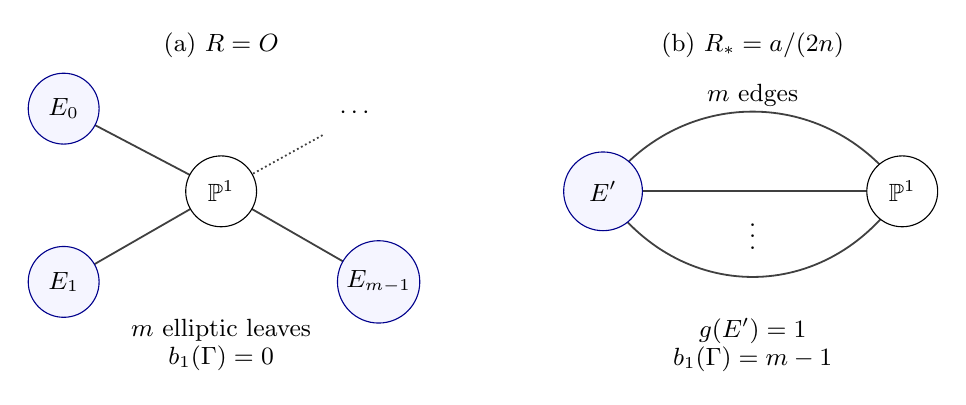
\begin{tikzpicture}[
  x=1cm,y=1cm,
  every node/.style={font=\small,inner sep=2pt},
  component/.style={draw,fill=white,circle,minimum size=9mm},
  elliptic/.style={component,draw=blue!55!black,fill=blue!4},
  edge/.style={draw=black!75,line width=.65pt}
]
  \node at (2.5,3.65) {\textup{(a)} $R=O$};
  \node at (9.25,3.65) {\textup{(b)} $R_*=a/(2n)$};

  \coordinate (rational) at (2.5,1.8);
  \coordinate (leafzero) at (.5,2.85);
  \coordinate (leafone) at (.5,.65);
  \coordinate (leaflast) at (4.5,.65);
  \draw[edge] (rational) -- (leafzero);
  \draw[edge] (rational) -- (leafone);
  \draw[edge] (rational) -- (leaflast);
  \draw[edge,densely dotted] (rational) -- (3.8,2.52);
  \node at (4.22,2.8) {$\cdots$};
  \node[component] at (rational) {$\mathbb P^1$};
  \node[elliptic] at (leafzero) {$E_0$};
  \node[elliptic] at (leafone) {$E_1$};
  \node[elliptic] at (leaflast) {$E_{m-1}$};
  \node[align=center] at (2.5,-.15)
    {$m$ elliptic leaves\\[-1pt] $b_1(\Gamma)=0$};

  \coordinate (emain) at (7.35,1.8);
  \coordinate (tail) at (11.15,1.8);
  \draw[edge] (emain) .. controls (8.3,3.15) and (10.2,3.15) .. (tail);
  \draw[edge] (emain) -- (tail);
  \draw[edge] (emain) .. controls (8.3,.35) and (10.2,.35) .. (tail);
  \node[fill=white,inner sep=1pt] at (9.25,1.33) {$\vdots$};
  \node[elliptic,minimum size=10mm] at (emain) {$E'$};
  \node[component] at (tail) {$\mathbb P^1$};
  \node at (9.25,3.02) {$m$ edges};
  \node[align=center] at (9.25,-.15)
    {$g(E')=1$\\[-1pt] $b_1(\Gamma)=m-1$};
\end{tikzpicture}

\caption{The dual graphs of the two special fibers.  Vertex labels
indicate component genera and identify the elliptic components; edges
are nodes.  At $R=O$ the graph is a star with $m$ elliptic leaves, so
the Jacobian is $E^m$.  At $R=a/(2n)$ two components meet in $m$
nodes, giving graph Betti number $m-1$.  The drawings are schematic
for general odd $m$.}
\label{geo:dual-graphs}
\end{figure}

The first degeneration has now supplied a split product fiber and a
neighborhood in which its homology can be compared with nearby smooth
fibers.  The second has supplied $m$ nodes, each with smoothing order
one.  We next identify their vanishing cycles in a single integral
basis.

\section{Integral homology and explicit monodromy}\label{sec:monodromy}

Fix the complex elliptic curve $E$ and the constant-$E$ family from
Section~\ref{sec:geometry}.  Let $n\geq3$ be odd and let $m>1$ divide
$n$.  We write
\[
 \Gamma_m=\mu_m,\qquad u:(Z,Y)\longmapsto(Z,e^{2\pi i/m}Y),
\]
so that $u$ is the chosen generator of the deck group.
Throughout this section $\Z[\Gamma_m]$ denotes the \emph{group ring}, not
the cyclotomic integer ring.  We first construct an integral basis
permuted by $u$, and then compute two monodromy operators in that same
basis.  Their reduction on character spaces will supply the residual
irreducibility used later.

\subsection{A basis obtained by cutting the torus}

Choose an oriented period basis $a,b$ and identify the underlying
oriented torus with $(\mathbb R/\Z)^2$, with $a$ horizontal and $b$ vertical.
Consider the path of parameters
\begin{equation}\label{mon:horizontal-path}
 R_s=\frac{s}{n}a,\qquad 0<s<\frac12.
\end{equation}
Its branch points are $-sa$ and $sa$.  Let $I_s$ be the horizontal arc
from $-sa$ to $sa$ through $O$.

\begin{lemma}\label{mon:slit}
For the parameters in \eqref{mon:horizontal-path}, the cover
$C_{m,R_s}\to E$ is trivial over $E\setminus I_s$.  It is obtained by
cutting $m$ copies of $E$ along $I_s$ and joining adjacent banks
cyclically.  Crossing the slit changes the sheet index by $1$ or $-1$,
according to the orientation of crossing and the initial choice of
indexing.
\end{lemma}

\begin{proof}
For small $s$, enclose the colliding sections in a small disk about
$O$.  The model at $R=O$ restricts outside that disk to $m$ disjoint
copies of its complement, by Proposition~\ref{geo:compact-type}.
If $D$ is such a disk, the inclusion
$E\setminus\operatorname{int}(D)\hookrightarrow E\setminus I_s$
is a homotopy equivalence.  The unramified cover of $E\setminus I_s$
is therefore trivial.  As $s$ varies in $(0,1/2)$, the arcs $I_s$ move by isotopy,
and the topological isomorphism class of this unramified cover remains
constant.  The monodromy around either branch point is a generator
of $\Gamma_m$, since its valuation in $f_R$ is $1$ or $-1$.
This gives the stated gluing.
\end{proof}

On each sheet let $a_i$ be the horizontal loop at vertical coordinate
$1/2$ and let $b_i$ be the vertical loop at horizontal coordinate
$1/2$, for $i\in\Z/m\Z$.  These loops avoid the slit, intersect at
one point on their common sheet, and may be oriented so that
\begin{equation}\label{mon:intersection}
 \langle a_i,b_j\rangle=\delta_{ij},\qquad
 \langle a_i,a_j\rangle=\langle b_i,b_j\rangle=0.
\end{equation}
Index the sheets so that $u$ sends $a_i,b_i$ to $a_{i+1},b_{i+1}$.

\begin{proposition}\label{mon:integral-module}
The cycles $a_i,b_i$ form an integral symplectic basis of
$H_1(C_{m,R_s},\Z)$.  Consequently, for every smooth fiber of the
family,
\begin{equation}\label{mon:free-lattices}
 H_1(C_m,\Z)\simeq\Z[\Gamma_m]^2,
 \qquad H^1(C_m,\Z)\simeq\Z[\Gamma_m]^2.
\end{equation}
In particular, after comparison, $H^1_{\mathrm{et}}(C_m,\Z_\ell)$ is
free of rank two over $\Z_\ell[\Gamma_m]$ for every prime $\ell$, including
$\ell\mid m$.
\end{proposition}

\begin{proof}
The genus is $m$, so $H_1$ has rank $2m$.  Equation~\eqref{mon:intersection}
shows that the $2m$ displayed classes are linearly independent and
span a sublattice with unimodular intersection pairing.  If its index
in $H_1$ were $d$, its intersection determinant would be $d^2$ times
the determinant on $H_1$.  Both determinants are $1$, so $d=1$.
The deck action now gives the first isomorphism in
\eqref{mon:free-lattices}.

The dual of the regular integral module is again regular: explicitly,
the coefficient-of-identity pairing
\[
 \Z[\Gamma_m]\times\Z[\Gamma_m]\longrightarrow\Z,
 \qquad (x,y)\longmapsto [1](xy)
\]
is perfect.  With the pullback action on the dual, it identifies
$\operatorname{Hom}_{\Z}(\Z[\Gamma_m],\Z)$ with $\Z[\Gamma_m]$.
This proves the cohomological assertion without dividing by $m$.
Topological local triviality transports the result through the connected
smooth parameter open, and comparison gives the \'etale assertion.
\end{proof}

\begin{remark}
The compact-type degeneration gives another explanation of the integral
statement.  Its Jacobian extends to an abelian scheme with special
fiber $E^m$, and $\Gamma_m$ permutes the factors regularly.
The integral homology of this fiber is the regular module twice.
The slit construction makes this description concrete by identifying
cycles that can also be followed towards the other degeneration.
\end{remark}

\subsection{Vanishing cycles and a common monodromy basis}

Let $s$ approach $1/2$ in \eqref{mon:horizontal-path}.  The branch
points meet at $a/2$, while the slit fills all but a shrinking gap in
the horizontal circle.  Choose a small disk about $a/2$ containing
both branch points, with radius larger than their distance from the
collision point.  Its boundary has $m$ closed lifts $\delta_i$.
They are the neck circles at the $m$ nodes of
Lemma~\ref{geo:collision}; hence they are the vanishing cycles.

\begin{lemma}\label{mon:vanishing-classes}
After a cyclic indexing of the lifts, their homology classes are
\begin{equation}\label{mon:delta}
 [\delta_i]=\pm(a_i-a_{i+1}),\qquad i\in\Z/m\Z,
\end{equation}
or the same formula with $i-1$ in place of $i+1$.
\end{lemma}

\begin{proof}
Arrange the boundary of the disk to cross the slit transversely twice.
A lifted boundary circle has its upper arc on one sheet and its lower
arc on an adjacent sheet.  Index the upper sheet by $i$; the lower
one is $i+1$ or $i-1$, by Lemma~\ref{mon:slit}.  The circle is disjoint
from every $a_j$.  It crosses the two corresponding vertical loops
once each, with opposite intersection signs, and no other $b_j$.
These intersections determine its class in the integral symplectic
basis of Proposition~\ref{mon:integral-module}, giving
\eqref{mon:delta}.  See Figure~\ref{mon:slit-figure}.
\end{proof}

\begin{figure}[tb]
\centering
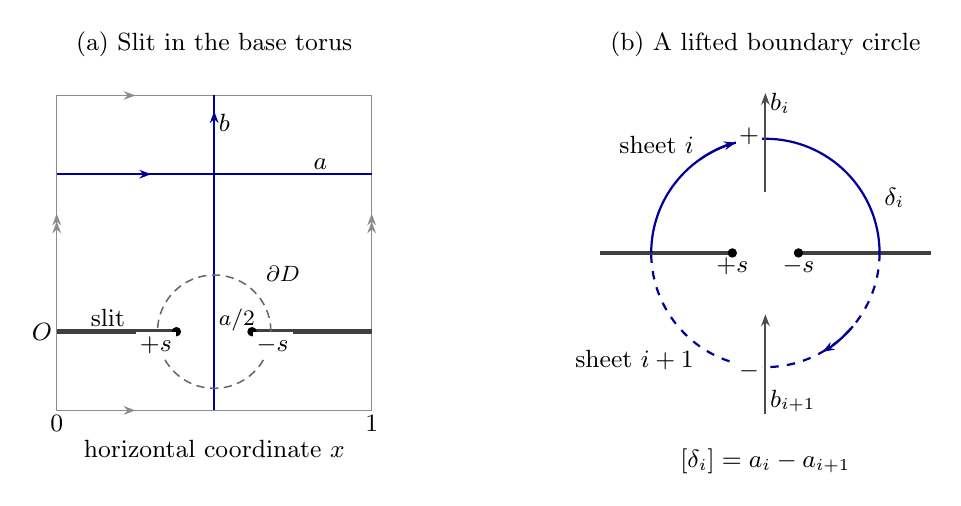
\begin{tikzpicture}[
  x=1cm,y=1cm,
  every node/.style={font=\small,inner sep=1.5pt},
  boundary/.style={draw=black!45,line width=.5pt},
  slit/.style={draw=black!75,line width=1.7pt},
  cycle/.style={draw=blue!60!black,line width=.8pt},
  arrow/.style={-{Stealth[length=1.5mm,width=1.1mm]}}
]
  \node at (2,4.65) {\textup{(a)} Slit in the base torus};
  \node at (9,4.65) {\textup{(b)} A lifted boundary circle};

  \draw[boundary] (0,0) rectangle (4,4);
  \draw[boundary,arrow] (.55,0) -- (1,0);
  \draw[boundary,arrow] (.55,4) -- (1,4);
  \draw[boundary,arrow] (0,2) -- (0,2.4);
  \draw[boundary,arrow] (4,2) -- (4,2.4);
  \draw[boundary,arrow] (0,2.1) -- (0,2.5);
  \draw[boundary,arrow] (4,2.1) -- (4,2.5);
  \node[below] at (0,0) {$0$};
  \node[below] at (4,0) {$1$};
  \node[below] at (2,-.32) {horizontal coordinate $x$};

  \draw[cycle] (0,3) -- (4,3);
  \draw[cycle,arrow] (.8,3) -- (1.2,3);
  \node[above] at (3.35,3) {$a$};
  \draw[cycle] (2,0) -- (2,4);
  \draw[cycle,arrow] (2,3.45) -- (2,3.8);
  \node[right] at (2,3.65) {$b$};

  \draw[slit] (0,1) -- (1.52,1);
  \draw[slit] (2.48,1) -- (4,1);
  \fill (1.52,1) circle (1.7pt);
  \fill (2.48,1) circle (1.7pt);
  \node[left] at (0,1) {$O$};
  \node[above] at (.65,1) {slit};
  \draw[densely dashed,black!60,line width=.55pt] (2,1) circle (.72);
  \node[below left,fill=white] at (1.52,1) {$+s$};
  \node[below right,fill=white] at (2.48,1) {$-s$};
  \node[above right,font=\footnotesize] at (2.6,1.58)
    {$\partial D$};
  \node[right,font=\footnotesize] at (2,1.15) {$a/2$};

  \draw[slit] (6.9,2) -- (8.58,2);
  \draw[slit] (9.42,2) -- (11.1,2);
  \fill (8.58,2) circle (1.7pt);
  \fill (9.42,2) circle (1.7pt);
  \node[below] at (8.58,2) {$+s$};
  \node[below] at (9.42,2) {$-s$};
  \draw[cycle] (7.55,2) arc[start angle=180,end angle=0,radius=1.45];
  \draw[cycle,dashed] (10.45,2) arc[start angle=0,end angle=-180,radius=1.45];
  \draw[cycle,arrow] (8.1683,3.1878)
    arc[start angle=125,end angle=105,radius=1.45];
  \draw[cycle,arrow] (10.1107,1.0679)
    arc[start angle=-40,end angle=-60,radius=1.45];
  \node[above left] at (8.15,3.2) {sheet $i$};
  \node[below left] at (8.15,.82) {sheet $i+1$};
  \node[right] at (10.45,2.7) {$\delta_i$};

  \draw[black!70,line width=.65pt,arrow] (9,2.78) -- (9,4.03);
  \draw[black!70,line width=.65pt,arrow] (9,-.05) -- (9,1.22);
  \node[right] at (9,3.9) {$b_i$};
  \node[right] at (9,.12) {$b_{i+1}$};
  \node[left,fill=white,inner sep=1pt] at (8.96,3.48) {$+$};
  \node[left,fill=white,inner sep=1pt] at (8.96,.5) {$-$};
  \node at (9,-.65) {$[\delta_i]=a_i-a_{i+1}$};
\end{tikzpicture}

\caption{The horizontal slit leaves a gap about the collision point
$a/2$.  A small circle about that gap crosses the slit twice.  Its
lift has one arc on sheet $i$ and the other on sheet $i+1$; its two
intersections with the lifted vertical cycles have opposite signs.
This identifies the vanishing class as $\pm(a_i-a_{i+1})$.
Opposite edges of the torus rectangle are identified; its coordinates
range over $[0,1]\times[-1/4,3/4]$, so $-s$ is plotted at $1-s$.
In the right panel, solid and dashed arcs distinguish the two sheets.}
\label{mon:slit-figure}
\end{figure}

\begin{theorem}\label{mon:transvections}
In one integral basis $a_i,b_i$ as above, the geometric monodromy of
the constant-$E$ family contains operators $T_a,T_b$ satisfying
\begin{align}
 T_a(a_j)&=a_j,&
 T_a(b_j)&=b_j+\sigma_a(2a_j-a_{j-1}-a_{j+1}),
 \label{mon:Ta}\\
 T_b(b_j)&=b_j,&
 T_b(a_j)&=a_j+\sigma_b(2b_j-b_{j-1}-b_{j+1}),
 \label{mon:Tb}
\end{align}
where $\sigma_a,\sigma_b\in\{1,-1\}$ are independent of $j$.
Equivalently, their two off-diagonal entries, in the basis of the free
$\Z[\Gamma_m]$-module, are $\sigma_a(2-u-u^{-1})$ and
$\sigma_b(2-u-u^{-1})$.
The geometric monodromy of the family over $U$ contains these actions
as well, under the pullback identification.
\end{theorem}

\begin{proof}
The Picard--Lefschetz formula for a positively oriented loop about a
semistable fiber is the product of the Dehn twists at its nodes;
see~\cite[Expos\'e~XV]{SGA7II}.  In the present family, every node
has smoothing order one by \eqref{geo:node-equation}, so every twist
has exponent one.  The vanishing cycles are disjoint.  Their
intersection pairings with one another therefore vanish, and the
product acts on a class $\gamma$ by
\begin{equation}\label{mon:PL}
 \gamma\longmapsto
 \gamma+\sigma\sum_i
 \langle\gamma,\delta_i\rangle[\delta_i],
\end{equation}
with one sign $\sigma$ depending only on the intersection convention.
Substituting \eqref{mon:delta} gives zero on the $a_j$ and, up to this
one sign,
\[
 (a_j-a_{j+1})-(a_{j-1}-a_j)
   =2a_j-a_{j-1}-a_{j+1}
\]
on $b_j$.  This proves \eqref{mon:Ta}.  Replacing the horizontal
path by $R_s=(s/n)b$ gives \eqref{mon:Tb}, initially in the basis
obtained from the corresponding vertical slit.

It remains to compare the two bases; this matters because separate
triangular matrices in unrelated bases would not give the stated
conclusion.  Choose the starting parameters of both paths sufficiently
close to $O$.  The horizontal loop at $y=1/2$ and the vertical loop
at $x=1/2$ avoid one fixed small disk about $O$ and avoid both short
slits.  Outside this disk the covering extends across $R=O$ as $m$
disjoint sheets.  Trivialize it over a small, simply connected
parameter disk containing $O$, and use this trivialization to label
the lifts of the two fixed loops.  Parallel transport between the
starting parameters now identifies both sets of $a_i,b_i$ with the
same basis.  There is no monodromy ambiguity from circling $O$ on
these classes: the sheet trivialization extends over $O$ itself.
A different initial labeling makes only a common cyclic shift, which
leaves \eqref{mon:Ta}--\eqref{mon:Tb} unchanged.

Both loops therefore define the asserted operators in a single
geometric monodromy group.  Pullback along the open parameter curve
in $E\to U$ maps its fundamental group into that of $U$, so these
operators occur in the latter image too.  Removing additional finitely
many points from either smooth parameter open induces a surjection
on fundamental groups and does not remove any of the operators.
\end{proof}

The operator $2-u-u^{-1}$ is the cyclic difference operator arising
from the adjacent-sheet vanishing classes.  The next sections use
the integral module in Proposition~\ref{mon:integral-module} to
specialize rotation characters, and the two matrices above to keep
the resulting residual representations irreducible.

\section{Rank-two systems and integral congruences}\label{sec:systems}

The cyclic covers now supply the Galois representations through which we
will transfer automorphy.  The involution identifies opposite rotation
characters, giving each character space the determinant and Hodge--Tate
weights of an elliptic curve.  The integral regular-module calculation
will then give congruences even at primes dividing the covering degree.

Return to an imaginary quadratic field $K$ and a non-CM elliptic curve
$E/K$.  By Serre's open image theorem \cite[\S4.4, Th\'eor\`eme~3]{SerreOpenImage}, choose a prime
$p>100$ such that the image of $G_K$ on $E[p]$ contains
$\SL_2(\F_p)$.  Set
\begin{equation}\label{sys:standing-fields}
 n=3p,\qquad F=K(\mu_n).
\end{equation}
Both $K/\Q$ and $\Q(\mu_n)/\Q$ are abelian, so $F/\Q$ is abelian.
It is a CM field: complex conjugation is central, its fixed field is
totally real, and $F$ has no real embedding because it contains $K$.
Moreover,
\begin{equation}\label{sys:no-fifth-roots}
 \zeta_5\notin F.
\end{equation}
Indeed, $\Q(\mu_n)$ is unramified at $5$, and the ramification index
of $F$ at $5$ is consequently at most $[K:\Q]=2$.  A field containing
$\Q(\zeta_5)$ has ramification index divisible by $4$ at $5$.

Apply the construction of Lemma~\ref{geo:family} with this $n$.
Write $U\subset\A^1_K$ for its parameter open and $B_t$ for the
quadratic twist of $E$ used there.  We may shrink $U$ whenever a smooth
proper model of one of the finitely many families is required.  Until
Section~\ref{sec:residual}, the point $t\in U(K)$ is arbitrary.

\subsection{Character spaces}

Fix an embedding $\overline\Q\hookrightarrow\C$ and put
$M=\Q(\mu_n)\subset\overline\Q$.  For each rational prime $\ell$, choose
an embedding
$j_\ell:\overline\Q\hookrightarrow\overline\Q_\ell$ and an isomorphism
$\iota_\ell:\overline\Q_\ell\xrightarrow{\sim}\C$ whose composition
with $j_\ell$ is the fixed complex embedding.  Every rotation character
in this section is a homomorphism
\[
 \theta:\mu_n(F)\longrightarrow M^\times.
\]
Write $C_m(t)=C_{m,t}$ for a fiber of the family.  For the curve
$C_n=C_n(t)$, define
\begin{equation}\label{sys:definition}
 V_{\theta,\ell}
 =\bigl\{x\in H^1_{\mathrm{\acute et}}
       (C_{n,\overline F},\overline\Q_\ell):
       u^*x=j_\ell(\theta(u))x\text{ for all }u\in\mu_n(F)\bigr\}.
\end{equation}
Here $u$ denotes the deck transformation with multiplier $u$.
All deck transformations are defined over $F$, so these are
$G_F$-representations.  We write $V_\theta$ for the collection of these
realizations.  In a congruence at $\ell$, all characters use the same
embedding $j_\ell$; this convention is essential when comparing their
reductions.

\begin{proposition}\label{sys:properties}
For every $t\in U(K)$ and every rotation character $\theta$, the
representations $V_{\theta,\ell}$ have the following properties.
\begin{enumerate}
\item They are semisimple of dimension two, with determinant
$\eps_\ell^{-1}$.
\item At every place of $F$ above $\ell$, they are potentially
semistable with labelled Hodge--Tate weights $\{0,1\}$.
\item There is a finite set of places $S$ of $F$, independent of
$\ell$, such that $V_{\theta,\ell}$ is unramified at every
$v\notin S$ of residue characteristic different from $\ell$.
At such a place its Frobenius characteristic polynomial is the image
under $j_\ell$ of a polynomial in $M[T]$ independent of $\ell$.
\end{enumerate}
\end{proposition}

\begin{proof}
The rank-two regular-module statement of
Proposition~\ref{mon:integral-module}, followed by comparison between
singular and \(\ell\)-adic cohomology, gives
$\dim V_{\theta,\ell}=2$.

Let $\langle\ ,\ \rangle$ be the cup-product pairing on $H^1(C_n)$,
with values in $\overline\Q_\ell(-1)$.  It pairs the $\theta$-space
perfectly with the $\theta^{-1}$-space.  The involution $w$ is defined
over $F$, preserves cup product, and exchanges these two spaces.
Consequently
\[
 [x,y]_\theta=\langle x,w^*y\rangle,
 \qquad x,y\in V_{\theta,\ell},
\]
is a perfect $G_F$-equivariant pairing into
$\overline\Q_\ell(-1)$.  It is alternating, because
\[
 \langle y,w^*x\rangle
   =\langle w^*y,x\rangle
   =-\langle x,w^*y\rangle.
\]
A perfect alternating pairing on a two-dimensional space identifies
its determinant with the target line.  This proves
$\det V_{\theta,\ell}=\eps_\ell^{-1}$.

To compute the Hodge numbers, make any embedding of $F$ into $\C$.
Let $a_\theta$ be the multiplicity of $\theta$ in the holomorphic
differentials of the resulting complex curve.  The holomorphic
involution $w$ gives $a_\theta=a_{\theta^{-1}}$.  Hodge decomposition
and complex conjugation identify the dimension of the full
$\theta$-space with $a_\theta+a_{\theta^{-1}}$.  Since this dimension
is two, $a_\theta=1$.  This argument works for every embedding and
every character.  The comparison theorems therefore give the labelled
weights $0,1$.  Potential semistability follows from semistable
reduction and the semistable comparison theorem for smooth proper
varieties; see \cite{Tsuji}.  These properties pass to the character
summands.

Outside a finite set, $C_n$ has good reduction and the rotations
extend to its smooth proper model.  Smooth proper base change gives
unramifiedness.  The projector onto the $\theta$-space is
\[
 e_\theta=\frac1n\sum_{u\in\mu_n(F)}
              j_\ell(\theta(u))^{-1}u^*.
\]
This formula is used only in characteristic zero.  The Lefschetz
trace formula for a rotation composed with a positive power of
Frobenius shows that its trace on $H^1(C_n)$ is independent of
$\ell$.  Applying the displayed projector gives traces in $M$,
compatible under the embeddings $j_\ell$.  Together with the
already determined determinant, this gives the asserted common
characteristic polynomial.

Finally, $H^1(C_n)$ is the first cohomology of its Jacobian.  Faltings'
semisimplicity theorem \cite[\S5, Satz~3]{Faltings} makes this a semisimple
$G_F$-representation.  Extension of scalars and passage to a
$G_F$-stable direct summand preserve semisimplicity, proving the
remaining assertion.
\end{proof}

\subsection{The two elliptic-curve realizations}

The characters of orders one and three will connect the new systems
to elliptic curves.  For the order-three character, the involution
produces a genus-one quotient rather than merely an abstract
rank-two summand.

\begin{proposition}\label{sys:elliptic}
If $\theta$ has order $m>1$ dividing $n$, the system $V_\theta$ is
realized by the corresponding character space in $H^1(C_m)$.
For the trivial character,
\[
 V_{1,\ell}\simeq H^1_{\mathrm{\acute et}}
                  (B_{t,\overline F},\overline\Q_\ell).
\]
Let $D_t=C_3(t)/\langle w\rangle$ and $A_t=\Jac(D_t)$.  Then $D_t$
has genus one, $A_t$ is an elliptic curve over $F$, and for either
nontrivial order-three character $\eta$ there are $G_F$-equivariant
isomorphisms
\[
 V_{\eta,\ell}\simeq
 H^1_{\mathrm{\acute et}}(A_{t,\overline F},\overline\Q_\ell)
 \qquad\text{for every }\ell.
\]
\end{proposition}

\begin{proof}
The quotient map $C_n\to C_m$ sends the covering coordinate $Y$ to
$Y^{n/m}$.  Pullback is injective on rational cohomology, since its
composition with trace is multiplication by the degree.  Its image
is the subspace fixed by the kernel of $\mu_n\to\mu_m$.
The rank-two calculation therefore identifies its order-$m$
character summand with $V_{\theta,\ell}$.  The same argument for the
quotient $C_n\to B_t$ identifies the trivial character space.

On $H^1(C_3)$, the trivial rotation space is $H^1(B_t)$, and $w$
acts there by $[-1]^*=-1$.  It exchanges the two nontrivial rotation
spaces, each of dimension two.  Their direct sum consequently has
a two-dimensional $w$-invariant subspace.  Rational cohomology of a
finite quotient is the invariant subspace, so
\[
 H^1(D_t)\simeq H^1(C_3)^{w=1}
\]
has dimension two.  Thus $D_t$ has genus one and its Jacobian is an
elliptic curve, whether or not $D_t$ has an $F$-rational point.
Projection of a vector $x+w^*x$ onto the $\eta$-space is $x$;
therefore this projection is a $G_F$-equivariant isomorphism from
the invariant subspace to $V_{\eta,\ell}$.  Finally,
$H^1(D_t)\simeq H^1(\Jac(D_t))$.  The latter identification is
independent of the geometric base point used in an Abel--Jacobi
map, because translations act trivially on cohomology.
\end{proof}

\subsection{Evaluation of the integral group ring}

A character projector contains the denominator $n$ and cannot by
itself establish a congruence at $3$ or $p$.  Instead, we use the
integral freeness proved in Section~\ref{sec:monodromy}.  Evaluation
of a free group-ring module gives a lattice before reduction; two
characters with the same residual values then give the same
residual representation.

\begin{lemma}\label{sys:integral-evaluation}
Fix $t\in U(K)$ and a prime $\ell$.  Let $L/\Q_\ell$ be a finite
extension containing $j_\ell(M)$, with ring of integers
$\mathcal O$, maximal ideal $\mathfrak m$, and residue field $k$.
For a rotation character $\theta$, the module
\[
 \mathcal T_\theta=
 H^1_{\mathrm{\acute et}}(C_{n,\overline F},\Z_\ell)
 \otimes_{\Z_\ell[\mu_n],\,j_\ell\theta}\mathcal O
\]
is a free rank-two $G_F$-stable lattice realizing
$V_{\theta,\ell}$ after extension to $\overline\Q_\ell$.
If $j_\ell\theta$ and $j_\ell\theta'$ have the same reduction as
characters $\mu_n\to k^\times$, then
\[
 \mathcal T_\theta/\mathfrak m\mathcal T_\theta
 \simeq
 \mathcal T_{\theta'}/\mathfrak m\mathcal T_{\theta'}
\]
as $k[G_F]$-modules.
\end{lemma}

\begin{proof}
By Proposition~\ref{mon:integral-module} and comparison,
\[
 H^1_{\mathrm{\acute et}}(C_{n,\overline F},\Z_\ell)
 \simeq \Z_\ell[\mu_n]^2
\]
as group-ring modules.  The Galois action commutes with this group
ring because the rotations are defined over $F$.  Tensoring by
evaluation at $j_\ell\theta$ therefore gives a free rank-two
$\mathcal O$-module with continuous Galois action.  In characteristic
zero the group algebra is semisimple; its quotient by character
evaluation is precisely the corresponding character summand.
This identifies its rational representation with $V_{\theta,\ell}$.

After reduction, the displayed tensor product becomes
\[
 H^1_{\mathrm{\acute et}}(C_{n,\overline F},\Z_\ell)
 \otimes_{\Z_\ell[\mu_n],\,\overline\theta} k.
\]
It depends only on the residual evaluation map
$\overline\theta$.  This proves the asserted isomorphism without
assuming that $\ell$ is prime to $n$.
\end{proof}

Choose a primitive character $\chi$ of order $n=3p$ and write its
unique primary decomposition as
\[
 \chi=\psi\eta,\qquad \operatorname{ord}(\psi)=p,
 \qquad \operatorname{ord}(\eta)=3.
\]
For a system $V_\theta$, write $\overline V_{\theta,\ell}$ for the
semisimplified reduction of a stable lattice, with scalars extended
to $\overline\F_\ell$.  This representation is independent of the
choice of stable lattice.

\begin{corollary}\label{sys:congruences}
For every $t\in U(K)$ there are isomorphisms
\begin{equation}\label{sys:congruence-chain}
 \overline V_{\eta,p}\simeq\overline V_{\chi,p},
 \qquad
 \overline V_{\chi,3}\simeq\overline V_{\psi,3},
 \qquad
 \overline V_{\psi,p}\simeq\overline V_{1,p}.
\end{equation}
These hold with the elliptic-curve realizations of
Proposition~\ref{sys:elliptic} at the two ends.
\end{corollary}

\begin{proof}
A root of unity of $\ell$-power order reduces to $1$ in residue
characteristic $\ell$.  Thus $\chi$ and $\eta$ have the same
reduction at $p$, $\chi$ and $\psi$ have the same reduction at $3$,
and $\psi$ and $1$ have the same reduction at $p$.
Lemma~\ref{sys:integral-evaluation} gives the three congruences.
The rational isomorphisms with the smaller covers and elliptic
curves in Proposition~\ref{sys:elliptic} preserve semisimplified
reduction, even if their natural integral pullbacks have index
divisible by $\ell$.
\end{proof}

The direction of propagation is now fixed: automorphy will pass
from $V_\eta$ to $V_\chi$ at $p$, then to $V_\psi$ at $3$, and
finally to $V_1$ at $p$.  The congruences themselves impose no
restriction on $t$.  The subsequent local and residual arguments will
choose one parameter for which all three automorphy-lifting steps apply.

\section{Automorphy inputs and the remaining specialization conditions}
\label{sec:inputs}

The congruences of Corollary~\ref{sys:congruences} connect the cohomology
of the auxiliary elliptic curve $A$ to that of the twist $B_t$ of $E$.
To turn them into a proof of automorphy, we use two results of
Caraiani--Newton. We state the precise forms needed here, and then identify
the properties that the parameter $t$ must satisfy. All the results quoted
from~\cite{CN} use the numbering of its third arXiv version.

\begin{definition}[Decomposed genericity]\label{def:decomposed-generic}
Let $L$ be a number field and let
$\overline r:G_L\to\GL_2(\overline\F_l)$ be continuous. The representation
is \emph{decomposed generic} if there is a rational prime $q\ne l$ splitting
completely in $L$ such that, for every $v\mid q$, it is unramified at $v$
and its Frobenius eigenvalues $\alpha_v,\beta_v$ satisfy
\[
 \alpha_v/\beta_v\ne q,\qquad \beta_v/\alpha_v\ne q
 \quad\text{in }\overline\F_l.
\]
\end{definition}

This is \cite[Definition~2.1.27]{CN}. Our construction will give
$q\equiv1\pmod l$, so it is enough to make the two eigenvalues distinct at
\emph{every} place above $q$.

We use potential ordinarity of Galois representations in the convention of
Section~\ref{sec:conventions}. The corresponding automorphic condition,
called \emph{$\iota$-ordinarity of weight zero}, is the ordinary Hecke
condition used in~\cite[Theorem~5.2]{CN}. It is imposed at a sufficiently deep
level and therefore allows ramified finite-order characters. We will obtain
it only for quadratic twists of Steinberg, using the local calculation in
\cite[Lemma~6.1.3(4)]{CN}.

\begin{theorem}[Caraiani--Newton, specialized form]\label{aut:lift}
Let $L$ be a CM number field and $l$ an odd prime other than $5$. Let
$r:G_L\to\GL_2(\overline\Q_l)$ be continuous, unramified outside finitely
many places, with determinant $\eps_l^{-1}$. Suppose that $r$ is potentially
semistable with labeled Hodge--Tate weights $0,1$ at every $v\mid l$,
that $\overline r$ is decomposed generic, and that
$\overline r|_{G_{L(\zeta_l)}}$ is absolutely irreducible.

Suppose there are a cuspidal weight-zero regular algebraic representation
$\pi$ of $\PGL_2(\A_L)$ and an isomorphism
$\iota:\overline\Q_l\xrightarrow{\sim}\C$ for which
$\overline{r_\iota(\pi)}\simeq\overline r$. At each $v\mid l$, assume one
of the following:
\begin{enumerate}[(i)]
\item Both local Galois representations are potentially crystalline;
one is potentially ordinary of weight zero if and only if the other is; and
$\rec_{L_v}(\pi_v)$ has zero monodromy.
\item Neither local Galois representation is potentially crystalline,
and $\pi$ is $\iota$-ordinary of weight zero at $v$.
\end{enumerate}
Then $r\simeq r_\iota(\Pi)$ for a cuspidal weight-zero regular algebraic
representation $\Pi$ of $\PGL_2(\A_L)$.
\end{theorem}

This is a sufficient-hypothesis specialization of
\cite[Theorem~5.2]{CN}. Its inverse-cyclotomic determinant hypothesis permits
$l=3$, including residual image $\SL_2(\F_3)$; see
\cite[Remark~5.2.2]{CN}. No additional residual adequacy assumption is being
made. All three applications below have $l=3$ or $l=p>100$.

\begin{theorem}[Elliptic starting point]\label{aut:seed}
Let $L$ be a CM number field not containing $\zeta_5$, and let $A/L$ be a
non-CM elliptic curve. If its mod-$5$ representation is decomposed generic
and is absolutely irreducible on $G_{L(\zeta_5)}$, then $H^1(A)$ is realized
by a cuspidal weight-zero regular algebraic representation of
$\PGL_2(\A_L)$.
\end{theorem}

This is \cite[Theorem~6.1 and Lemma~6.1.3]{CN}, after dualizing the Tate-module
convention there when necessary. Absolute irreducibility and decomposed
genericity in dimension two are preserved by duality.

For later use we also record the compatibility available after an elliptic
curve itself is known to be modular.

\begin{theorem}[Compatibility for modular elliptic curves]
\label{aut:elliptic-compat}
Let $D/L$ be a non-CM elliptic curve over a CM number field. Suppose that a
regular algebraic cuspidal representation $\pi$ realizes $H^1(D)$ at one
coefficient prime. Then $\pi$ has weight zero and trivial central character,
realizes $H^1(D)$ at every coefficient prime and every coefficient
isomorphism, and satisfies
\[
 \iota\WD\bigl(H^1(D,\overline\Q_l)|_{G_{L_v}}\bigr)^{\Fss}
 \simeq\rec^T_{L_v}(\pi_v)\qquad(v\nmid l).
\]
If $D$ has potentially multiplicative reduction at $v\mid l$, then $\pi$
is $\iota$-ordinary of weight zero there.
\end{theorem}

This is \cite[Lemma~6.1.3]{CN}. For the intermediate systems, which need not
come from elliptic curves, we use instead the general existence and
good-place compatibility of $r_\iota(\pi)$ from~\cite{HLTT,Scholze}, and
Varma's equality of the underlying semisimplified Weil representations at
$v\nmid l$~\cite[Theorem~1]{Varma}. The local reduction analysis in
Section~\ref{sec:local} will supply the additional facts needed in
Theorem~\ref{aut:lift}.

Here is what remains to be arranged for a single parameter $t\in U(K)$.
The determinant and Hodge--Tate conditions hold for every parameter by
Proposition~\ref{sys:properties}. At places above $3p$, we will make the
Jacobian of $C_n(t)$ potentially good ordinary, potentially good with all
Newton slopes $1/2$, or potentially totally toric, according to the
reduction type of $E$. This will make all four systems potentially
crystalline and potentially ordinary, potentially crystalline but not potentially ordinary, or
non-potentially crystalline, respectively. Section~\ref{sec:local} obtains
these properties from nonempty local open conditions on $t$.

Section~\ref{sec:residual} then chooses a parameter in those open sets for
which the residual hypotheses hold. The pairs $(m,l)=(3,5),(3,p),(p,3)$
provide respectively the elliptic starting point and the first two lifts;
the last lift uses the large mod-$p$ image of $E$. The two conjugates of
$K$ must be considered together to obtain decomposed genericity. Once
these properties have been proved, Section~\ref{sec:automorphy} propagates
automorphy along the three congruences and descends to $K$.

\section{Prescribing the local reduction type}\label{sec:local}

The degeneration at the origin allows us to arrange the same local behavior
for every character summand of the covering curve.  We first explain why the
reduction type of an abelian variety is controlled, locally in a
characteristic-zero family, by a sufficiently large finite torsion module.
We then apply this observation to the Jacobian family and translate its
reduction into the local conditions on the two-dimensional representations.

\subsection{Finite torsion and reduction in a local family}

Throughout this section, a local field is a finite extension of
$\Q_\ell$.  In this subsection, the auxiliary torsion prime $d$ is different
from $\ell$.  If $A$ is an abelian variety, write
$V_d(A)=T_d(A)\otimes_{\Z_d}\Q_d$ for its rational Tate module.

\begin{lemma}[Local constancy of finite torsion]\label{loc:torsion}
Let $L$ be a local field, let $X$ be a smooth $L$-variety, and let
$\mathcal A\to X$ be an abelian scheme.  For $x_0\in X(L)$ and an integer
$N\geq 1$, there is an analytic neighborhood $\mathcal N$ of $x_0$ in
$X(L)$ such that
\[
 \mathcal A_x[N](\overline L)\simeq
 \mathcal A_{x_0}[N](\overline L)
 \qquad (x\in\mathcal N)
\]
as $G_L$-modules.
\end{lemma}

\begin{proof}
The group scheme $\mathcal A[N]$ is finite \'{e}tale over $X$, since the
base has characteristic zero.  Equivalently, the scheme of full level-$N$
structures is a finite \'{e}tale torsor over $X$ under the constant group
$\GL_{2g}(\Z/N\Z)$, where $g$ is the relative dimension.
Choose a finite Galois extension $L'/L$ over which the fiber of this torsor
at $x_0$ splits.  The inverse function theorem for an \'{e}tale morphism gives
a local section through each point of the fiber over a neighborhood of
$x_0$ in $X(L')$.  Shrinking that neighborhood, these sections enumerate
all points in every nearby fiber.  Intersecting its finitely many Galois
conjugates, and shrinking once more if necessary, makes the neighborhood
Galois stable and preserves the Galois permutations of the sections.
The right action of the finite level group likewise preserves the same
permutations after shrinking.  Restricting to $X(L)$ therefore identifies
the fibers as Galois sets with their level-group action, and hence
identifies the underlying torsion modules.
\end{proof}

The finite torsion module will first ensure semistability and then
identify a Frobenius polynomial.  For the second step we use the
polynomial on the \emph{full} Tate module: this retains both the toric and
the lattice pieces of the semistable representation.

\begin{lemma}[Finitely many semistable Frobenius polynomials]
\label{loc:frobenius}
Fix a local field $L$ with residue field of cardinality $Q$, an integer
$g\geq 1$, and a prime $d$ different from the residue characteristic.
For a semistable abelian variety $A/L$ of dimension $g$, let
\[
 P_A(T)=\det\bigl(T-\operatorname{Frob}_L\mid V_d(A)\bigr),
\]
where $\operatorname{Frob}_L$ is any lift of arithmetic Frobenius.
Then $P_A(T)$ belongs to $\Z[T]$, is independent of the lift and of $d$,
and ranges over a finite set depending only on $g$ and $Q$.
Moreover, $P_A$ determines the toric rank of $A$; if that rank is zero,
it also determines the Newton polygon of its good reduction.
\end{lemma}

\begin{proof}
Let $r$ be the toric rank of $A$.  The semistable filtration of
Grothendieck identifies the graded pieces of $V_d(A)$ with the rational
Tate module of a torus of rank $r$, the rational Tate module of an abelian
variety of dimension $g-r$ with good reduction, and a lattice of rank $r$
\cite[Expos\'e IX]{SGA7I}.  The character lattice of the torus and the lattice quotient have finite
unramified Galois action.  Consequently the arithmetic Frobenius eigenvalues on the toric and
lattice graded pieces are respectively $Q$ times roots of unity and
roots of unity.  The middle
piece has the $2(g-r)$ Frobenius eigenvalues of an abelian variety over
$\F_Q$, all of complex absolute value $Q^{1/2}$.

Each graded piece has an integral characteristic polynomial independent
of $d$: for the toric and lattice pieces this follows from the finite-order
integral actions just described, together with the toric Tate twist;
for the abelian piece it is the
usual finite-field Frobenius polynomial.  Inertia acts trivially on the
graded pieces, so the product of these three polynomials is also
independent of the lift of Frobenius.  Every root has complex absolute
value at most $Q$.  Thus the coefficient of $T^{2g-j}$ has absolute value
at most $\binom{2g}{j}Q^j$.  Integral polynomials of fixed degree with
these bounds form a finite set.

Exactly $r$ roots have absolute value $1$, exactly $r$ have absolute value
$Q$, and the others have absolute value $Q^{1/2}$.  Since $Q>1$, these
three absolute values distinguish $r$.  If $r=0$, semistability is good
reduction, and the normalized $\ell$-adic valuations of the roots of
$P_A$ are its Newton slopes.
\end{proof}

\begin{proposition}[Local constancy of the semistable type]
\label{loc:constancy}
Let $L_0$ be a local field, let $X$ be a smooth $L_0$-variety, and let
$\mathcal A\to X$ be an abelian scheme of relative dimension $g$.
For $x_0\in X(L_0)$, there exist a finite extension $L/L_0$ and an analytic
neighborhood $\mathcal N\subset X(L_0)$ of $x_0$ with the following
properties.  For every $x\in\mathcal N$, the abelian variety
$\mathcal A_x$ is semistable over $L$ and has the same toric rank as
$\mathcal A_{x_0}$ over $L$.  If $\mathcal A_{x_0}$ has good reduction
over $L$, then $\mathcal A_x$ has the same Newton polygon over $L$.

In particular, if $\mathcal A_{x_0}\simeq E_0^g$ for an elliptic curve
$E_0/L_0$, every sufficiently nearby fiber has, after the same finite
extension, the same one of the following three properties as $E_0^g$:
\begin{enumerate}
\item good ordinary reduction;
\item good reduction with all Newton slopes equal to $1/2$;
\item semistable reduction of toric rank $g$.
\end{enumerate}
\end{proposition}

\begin{proof}
Choose an odd prime $d$ different from the residue characteristic.
By semistable reduction, we may choose a finite extension $L/L_0$ over
which $\mathcal A_{x_0}$ is semistable and all its $d$-torsion points are
rational.  Lemma~\ref{loc:torsion}, applied after base change to $L$,
shows that, in a neighborhood of $x_0$, all nearby fibers also have
rational $d$-torsion over $L$.

These fibers are semistable over $L$.  Indeed, the matrix of any inertia
element on their $d$-adic Tate module has the form $1+dB$ with $B$
integral.  Each eigenvalue $\lambda$ therefore satisfies
$v_d(\lambda-1)\geq 1$, where $v_d(d)=1$.  The local monodromy theorem
makes $\lambda$ a root of unity.  For odd $d$ the only root of unity
satisfying this inequality is $1$: a root with nontrivial prime-to-$d$ part has
$v_d(\lambda-1)=0$, and a primitive $d^a$th root has valuation
$1/(d^{a-1}(d-1))<1$.  Thus every inertia element acts unipotently, and
Grothendieck's criterion gives semistability
\cite[Expos\'e IX]{SGA7I}.

Let $\mathcal P$ be the finite set of polynomials in
Lemma~\ref{loc:frobenius} for dimension $g$ and the residue cardinality
of $L$.  Choose $j$ so large that reduction modulo $d^j$ is injective on
$\mathcal P$.  A second application of Lemma~\ref{loc:torsion} gives,
throughout a smaller neighborhood,
\[
 \mathcal A_x[d^j](\overline L)\simeq
 \mathcal A_{x_0}[d^j](\overline L)
 \quad\text{as }G_L\text{-modules}.
\]
Their full Frobenius polynomials are congruent modulo $d^j$, hence equal.
Lemma~\ref{loc:frobenius} now gives the assertions about toric rank and
Newton polygon.  The inverse image of this neighborhood under
$X(L_0)\to X(L)$ is a neighborhood of $x_0$, as required.

For the final assertion, choose $L$ so that $E_0$ has good or split
multiplicative reduction.  In the good case an elliptic curve is either
ordinary or supersingular; in the latter case both its Newton slopes
are $1/2$.  In the multiplicative case $E_0^g$ has toric rank $g$.
Enlarging $L$ to rationalize its $d$-torsion preserves these properties,
so the preceding argument applies.
\end{proof}

\subsection{Monodromy of a totally toric abelian variety}

The third possibility in Proposition~\ref{loc:constancy} must force
nonzero monodromy on \emph{each} character summand, including when the
coefficient prime is the residue characteristic.  The rank statement
needed for this is a consequence of the valuation pairing in toric
uniformization.  We give the argument at the residue characteristic as
well, in terms of Kummer extensions.

\begin{lemma}\label{loc:toric-monodromy}
Let $L/\Q_\ell$ be finite and let $A/L$ be an abelian variety of
dimension $g$.  Suppose that $A$ acquires semistable
reduction of toric rank $g$ after a finite extension.  For every prime
$d$, the monodromy operator on the Weil--Deligne representation of
$H^1_{\mathrm{et}}(A_{\overline L},\Q_d)$ has rank $g$.
For $d=\ell$, the Weil--Deligne representation is the one attached to
the potentially semistable representation by $\ell$-adic Hodge theory.
\end{lemma}

\begin{proof}
Monodromy rank does not change after finite extension.  We may therefore
assume that $A$ has split toric uniformization
\[
 A^{\mathrm{an}}\simeq (\Gm^g)^{\mathrm{an}}/\Lambda,
\]
where $\Lambda\simeq\Z^g$ is rational over $L$.  Choosing bases of the
torus and lattice writes the periods as a matrix
$(q_{ij})\in(L^\times)^{g\times g}$.  The valuation pairing is
nondegenerate, so
\begin{equation}\label{loc:valuation-matrix}
 \bigl(v_L(q_{ij})\bigr)_{1\leq i,j\leq g}
 \quad\text{is nonsingular.}
\end{equation}
This is the toric case of the monodromy pairing for a semistable
abelian variety \cite[Expos\'e IX]{SGA7I}; its realization on de Rham
cohomology is described in \cite{ColemanIovita}.

If $d\ne\ell$, the same pairing describes the monodromy map from the
lattice quotient to the toric subspace of the Tate module.  Its
nondegeneracy gives rank $g$.  We now prove this rank assertion for
$d=\ell$.

Toric uniformization supplies an exact sequence
\begin{equation}\label{loc:tate-extension}
 0\longrightarrow\Q_\ell(1)^g\longrightarrow V_\ell(A)
   \longrightarrow\Q_\ell^g\longrightarrow0,
\end{equation}
whose extension classes are the Kummer classes of the $q_{ij}$.
The representation is semistable, by the semistable comparison theorem
for abelian varieties \cite{ColemanIovita}.  Let $L_{\mathrm{ur}}$ be the
maximal unramified subfield of $L$, and write
$D_{\mathrm{st}}$ for Fontaine's semistable functor over $L$.
On the two outer terms of~\eqref{loc:tate-extension}, monodromy is zero.
Consequently it induces a map
\[
 \nu:D_{\mathrm{st}}(\Q_\ell^g)
       \longrightarrow D_{\mathrm{st}}(\Q_\ell(1)^g).
\]
After the standard identifications, Frobenius on these two spaces is
respectively $\sigma$ and $\ell^{-1}\sigma$, with $\sigma$ the Frobenius
of $L_{\mathrm{ur}}/\Q_\ell$.  The identity $N\varphi=\ell\varphi N$
therefore makes $\ker\nu\subset L_{\mathrm{ur}}^g$ stable under $\sigma$.

Suppose that $\nu$ has rank less than $g$.  Finite Galois descent for
$L_{\mathrm{ur}}/\Q_\ell$ then gives a nonzero vector
$a=(a_j)\in\Q_\ell^g\cap\ker\nu$.
Pull~\eqref{loc:tate-extension} back along the line spanned by $a$ in
its trivial quotient.  The resulting extension of $\Q_\ell$ by
$\Q_\ell(1)^g$ is semistable and has zero monodromy, hence is crystalline.
Under Kummer theory the Bloch--Kato crystalline subspace
$H_f^1(L,\Q_\ell(1))$ is the kernel of the valuation map
\cite[Example~3.9]{BlochKato}.  Applying this to each coordinate of the
pulled-back extension gives
\[
 \sum_{j=1}^g a_jv_L(q_{ij})=0
 \qquad(1\leq i\leq g),
\]
contrary to~\eqref{loc:valuation-matrix}.
Thus $N$ has rank $g$ on $V_\ell(A)$.  Dualizing gives the same rank
on $H^1_{\mathrm{et}}(A_{\overline L},\Q_\ell)$.
\end{proof}

\subsection{Open conditions on the original parameter}

Return to the elliptic curve $E/K$, the odd integer $n=3p$, and
$F=K(\mu_n)$.  The Jacobian of the constant-$E$ cover $C_n$ extends over
a neighborhood of $O$ in the parameter curve $E$, with fiber $E^n$ at
$O$, by Proposition~\ref{geo:compact-type}.  Proposition~\ref{loc:constancy}
therefore applies at every finite completion of $F$.  The following statement
expresses the resulting neighborhoods in the original parameter
$t\in U\subset\A^1_K$, so they can later be combined with Hilbert
irreducibility.

\begin{proposition}\label{loc:opens}
For every place $v_0\mid 3p$ of $K$, there is a nonempty open subset
$\Omega_{v_0}\subset U(K_{v_0})$ with the following property.
Suppose that $t\in U(K)$ belongs to $\Omega_{v_0}$ for all $v_0\mid3p$,
and set $J_t=\Jac(C_{n,t})$.  At each place $v\mid3p$ of $F$,
$J_t$ has the same one of the following potential reduction types
as $E^n$:
\begin{enumerate}
\item good ordinary reduction;
\item good reduction with all Newton slopes $1/2$;
\item semistable reduction of toric rank $n$.
\end{enumerate}
For each $v$, the extensions giving these properties may be chosen
in advance, independently of $t$ in the indicated open subsets.
\end{proposition}

\begin{proof}
Fix $v_0\mid3p$.  For each $v\mid v_0$, apply
Proposition~\ref{loc:constancy} to the extended Jacobian family over
$F_v$, at the point $O$ of its parameter curve.  This gives a
neighborhood of $O$ in $E(F_v)$ and a fixed finite extension of $F_v$
on which the asserted reduction type holds.  The inverse images of
these finitely many neighborhoods in $E(K_{v_0})$ have an intersection
that is again a neighborhood of $O$.

Choose $R_0\ne O$ in this intersection, sufficiently close to $O$ and
away from the finitely many excluded parameters of the cover family.
We may also avoid the ramification points of
$x:E\to\mathbf P^1$, since these form a finite set.  The local inverse
function theorem gives a nonempty neighborhood
$\Omega_{v_0}\subset U(K_{v_0})$ of $x(R_0)$ and an analytic lift
\[
 R(t)=(t,y(t))\in E(K_{v_0}),\qquad y(t)^2=h(t),
\]
whose image remains in the chosen intersection.  Shrink the neighborhood
so that $y(t)\ne0$ and it avoids all excluded parameters.

The map
\[
 B_t\longrightarrow E,\qquad (x,y)\longmapsto(x,y(t)y)
\]
is an isomorphism over $K_{v_0}$ carrying the marked point $(t,1)$ to
$R(t)$.  It carries the defining function for the cover to the function
in the constant-$E$ construction: their divisors agree, and both have
value $1$ at $O$.  Thus it identifies the covers and their Jacobians at
every $v\mid v_0$.  The reduction conclusions follow from the choice of
the neighborhoods.  Carrying this out independently at the finitely
many $v_0\mid3p$ proves the proposition.
\end{proof}

\subsection{The local representations of the character summands}

For a prime $\ell$ and a rotation character $\theta$, write
$V_{\theta,\ell}$ for the $\ell$-adic realization of the rank-two system
in Section~\ref{sec:systems}.  Recall from Section~\ref{sec:conventions} that the ordinary
filtration of weight zero has an unramified character on its line and
$\eps_\ell^{-1}$ times an unramified character on its quotient, after
a finite extension.  In the ordinary case below the distinguished
line is already preserved before this extension.

\begin{corollary}\label{loc:characters}
Choose $t$ satisfying the open conditions of
Proposition~\ref{loc:opens}.  Let $v\mid3p$ be a place of $F$, of residue
characteristic $\ell$.  Then, simultaneously for every rotation
character $\theta$, the following conclusions hold.
\begin{enumerate}
\item If $E$ has potentially good ordinary reduction at $v$, then
$V_{\theta,\ell}|_{G_{F_v}}$ is potentially crystalline and potentially
ordinary of weight $0$.
\item If $E$ has potentially good supersingular reduction at $v$, then
$V_{\theta,\ell}|_{G_{F_v}}$ is potentially crystalline and is not
potentially ordinary of weight $0$.
\item If $E$ has potentially multiplicative reduction at $v$, then the
monodromy of $V_{\theta,d}|_{G_{F_v}}$ has rank one for every coefficient
prime $d$, including $d=\ell$.  In particular,
$V_{\theta,\ell}|_{G_{F_v}}$ is not potentially crystalline.
\end{enumerate}
\end{corollary}

\begin{proof}
Choose a finite extension $L/F_v$ on which $J_t$ has the reduction given
by Proposition~\ref{loc:opens}.  In the two good-reduction cases,
crystalline comparison makes $H^1_{\mathrm{et}}(J_{t,\overline L},\Q_\ell)$,
and hence each character summand, crystalline over $L$.

Suppose first that the reduction is ordinary.  The connected--\'{e}tale
sequence of the ordinary $\ell$-divisible group, dualized to $H^1$, gives
a filtration whose subrepresentation is unramified and whose quotient
is $\eps_\ell^{-1}$ times an unramified representation.  This filtration
is functorial in endomorphisms and therefore stable under the rotations.
It restricts to such a filtration on each $V_{\theta,\ell}$.
By Proposition~\ref{sys:properties}, this summand has dimension two
and labeled Hodge--Tate weights $0,1$.  Its unramified part contributes
only weight $0$, whereas the quotient contributes only weight $1$;
thus both parts have dimension one.  This is the required ordinary
filtration.  After replacing $L$ by a finite Galois extension, its
weight-zero line is uniquely determined by its inertia action, since
$\eps_\ell$ has infinite image on the inertia of every finite extension.
Conjugation by $G_{F_v}$ preserves that line, so the line descends to
the original decomposition group.

If the reduction has all slopes $1/2$, the crystalline module of every
summand has the same slope.  These normalized slopes remain $1/2$
after further finite extension.  An ordinary filtration of weight $0$
would provide a crystalline rank-one subrepresentation of parallel
Hodge--Tate weight zero.  For that character weak admissibility forces
Newton slope zero, contradicting the slopes of the summand.  Thus no
such potential ordinary filtration exists.

Finally, suppose that $J_t$ has potentially toric rank $n$.
Lemma~\ref{loc:toric-monodromy} gives rank $n$ for monodromy on its
$2n$-dimensional first cohomology, at every coefficient prime.
Monodromy commutes with the rotations, so preserves the $n$ character
summands.  Each summand has dimension two.  On first cohomology of a
semistable abelian variety one has $N^2=0$, so the rank on each summand
is at most one.  Their ranks sum to $n$ and there are exactly $n$
summands; every rank is therefore one.  Nonzero monodromy persists
after finite extension and excludes potential crystallinity.
\end{proof}

\section{One specialization with all residual properties}\label{sec:residual}

We now choose a single parameter for the congruence chain.  The geometric
monodromy supplies irreducibility and suitable Frobenius elements, whereas
Hilbert irreducibility allows us to retain these elements after imposing
the local conditions of Section~\ref{sec:local}.  To obtain decomposed
genericity, we must control every place above a split rational prime.
We therefore specialize the two conjugate parameter families together.

Throughout this section, $K,E,p,n,F,U$ have the meanings fixed in
Section~\ref{sec:systems}.  In particular, $p>100$, $n=3p$, and
$F=K(\mu_n)$.  The pairs of covering degree and residual characteristic
that require geometric monodromy are
\begin{equation}\label{res:pairs}
 (m,\ell)=(3,p),\quad(3,5),\quad(p,3).
\end{equation}
In each case $\ell\nmid m$, so the residual cohomology decomposes into
rotation-character spaces after extending its finite coefficient field.

\subsection{Consequences of the two monodromy transformations}

\begin{lemma}\label{res:geometric}
For each pair in \eqref{res:pairs}, the geometric monodromy of
$H^1(C_m,\overline\F_\ell)$ on every nontrivial rotation-character
space is absolutely irreducible.  Its image contains opposite
nonidentity root unipotents on that space.  Moreover, one element
of the geometric monodromy acts regular semisimply on all these
nontrivial character spaces simultaneously.
These statements also hold for the conjugate family over $K$.
\end{lemma}

\begin{proof}
We first work with homology; duality will give the cohomological
statements.  On the character space with generator eigenvalue
$\lambda\in\overline\F_\ell^\times$, the transformations of
Theorem~\ref{mon:transvections} have the form
\[
 T_a=\begin{pmatrix}1&\sigma c_\lambda\\0&1\end{pmatrix},
 \qquad
 T_b=\begin{pmatrix}1&0\\\tau c_\lambda&1\end{pmatrix},
 \qquad
 c_\lambda=2-\lambda-\lambda^{-1},
\]
where $\sigma,\tau\in\{1,-1\}$.  Since
$c_\lambda=-(\lambda-1)^2/\lambda$, it is nonzero when
$\lambda\ne1$.  The two matrices have different unique invariant
lines, even over the algebraic closure.  Hence their common
representation is absolutely irreducible.

The product $T_aT_b^k$ has determinant one and trace
\begin{equation}\label{res:trace-product}
 2+\sigma\tau k c_\lambda^2.
\end{equation}
In odd characteristic, a determinant-one matrix is regular
semisimple exactly when its trace is different from $2$ and $-2$.
If $m=3$, then $\lambda+\lambda^{-1}=-1$, so $c_\lambda=3$ for both
nontrivial characters.  Take $k=2$.  The two possible traces in
\eqref{res:trace-product} are $20$ and $-16$.  Modulo $5$ these
are $0$ and $4$, and neither equals $2$ or $-2$; modulo $p>100$
they again avoid $2$ and $-2$.

For $m=p$ and $\ell=3$, take $k=1$.  Failure of regular
semisimplicity would force $c_\lambda^2=4$ or $-4$, since
$c_\lambda\ne0$.  Multiplying either equation by $\lambda^2$
gives a polynomial of degree four over $\F_3$ satisfied by
$\lambda$.  Its degree over $\F_3$ is therefore some $d\le4$,
and its order divides $3^d-1\le80$.  This contradicts the fact
that its order is the prime $p>100$.  Thus the same product works
for every nontrivial character in this case as well.

The transformations come from loops in the constant-elliptic-curve
parameter space.  As explained in Theorem~\ref{mon:transvections},
that family is a pullback of the family over $U$.  Its monodromy
image is therefore contained in the geometric monodromy image
over $U$.  Duality preserves absolute irreducibility, nonidentity
unipotents, and regular semisimplicity.  This proves the assertions
for cohomology.  The geometric argument applies to every complex
elliptic curve, so it applies equally to the conjugate of $E$.
\end{proof}

\subsection{The original elliptic curve and its conjugate}

The trivial character requires a different argument, since the
geometric family varies only a quadratic twist of $E$.  Its large
residual image was built into the choice of $p$.  The following
count shows that no independence assumption between $E$ and its
conjugate is necessary.

\begin{lemma}\label{res:trivial-character}
For every $t\in U(K)$, the representation
$\overline V_{1,p}$ is absolutely irreducible on $G_{F(\zeta_p)}$
and is decomposed generic over $F$.
\end{lemma}

\begin{proof}
Let $\Gamma$ be the image of $G_K$ on $E[p]$.
The abelian extension $F/K$ implies that the image of $G_F$
contains $[\Gamma,\Gamma]$.  Since $\Gamma$ contains
$\SL_2(\F_p)$ and this group is perfect for $p>3$, its commutator
subgroup is $\SL_2(\F_p)$: one inclusion follows from
perfectness, and the other from the determinant map.
Moreover, the determinant is trivial on $G_F$ because
$\mu_p\subset F$.  We have therefore proved
\begin{equation}\label{res:SL2-image}
 \rho_{E,p}(G_F)=\SL_2(\F_p).
\end{equation}
The same equality holds for the conjugate curve $E^c$, where $c$
is the nontrivial automorphism of $K/\Q$, because $F/\Q$ is normal.

Consider the joint image
\[
 J\subset\SL_2(\F_p)\times\SL_2(\F_p)
\]
of $G_F$ on $E[p]$ and $E^c[p]$.  Both projections are surjective.
In $\SL_2(\F_p)$ there are exactly $p^2$ matrices of trace $2$.
Indeed, writing a matrix as $\left(\begin{smallmatrix}a&b\\c&d
\end{smallmatrix}\right)$, the trace and determinant conditions
give $d=2-a$ and $bc=-(a-1)^2$.  The value $a=1$ gives $2p-1$
choices for $(b,c)$; the other $p-1$ values of $a$ each give
$p-1$ choices.  Their sum is $p^2$.  Replacing a matrix by its
negative gives the same count for trace $-2$.

The order of $\SL_2(\F_p)$ is $p(p^2-1)$.  Since each projection
of $J$ has equal-sized fibers, the proportion of elements of $J$
whose image in at least one factor has trace $2$ or $-2$ is at most
\[
 2\frac{2p^2}{p(p^2-1)}
 =\frac{4p}{p^2-1}<1.
\]
Thus some element of $G_F$ acts regular semisimply on both
$E[p]$ and $E^c[p]$.

Take a finite Galois extension of $\Q$ containing $F$ and the
fields needed for these two residual actions.  Conjugation by
$G_\Q$ either preserves the two curves or exchanges them, and
conjugates their residual matrices.  The selected element and all
its conjugates therefore act regular semisimply on the
representation of $E$.  Chebotarev supplies rational primes $q$
splitting completely in $F$ with this property at every $v\mid q$
of $F$.  We exclude $p$ and the finitely many primes of bad
reduction.  Since $\mu_p\subset F$, these primes satisfy
$q\equiv1\pmod p$.  Distinct Frobenius eigenvalues then give the
ratio condition in the definition of decomposed genericity.

The curve $B_t$ is a quadratic twist of $E$.  Twisting multiplies
residual matrices by scalar signs and hence preserves absolute
irreducibility and eigenvalue ratios.  Excluding the finitely many
ramified primes of this twist leaves the same Chebotarev argument
available.  Finally, $\zeta_p\in F$, and taking the dual of $E[p]$
gives the residual $H^1$ realization.  Proposition~\ref{sys:elliptic}
now proves both assertions for $\overline V_{1,p}$.
\end{proof}

\subsection{Simultaneous specialization}

We have obtained the requisite geometric elements and dealt with
the trivial character.  It remains to retain the geometric elements
at one parameter and arrange that their Frobenius properties hold
at all places above a rational prime.  Restriction of scalars makes
the two conjugate parameter families visible in the same finite
Galois cover.

We next record precisely the specialization theorem needed to
preserve these finite monodromy images.  Allowing a constant field
in the cover is essential: the Frobenius primes used below must
split in a prescribed field.

\begin{lemma}\label{res:finite-specialization}
Let $W$ be a nonempty open subset of $\A^d_\Q$, let $D/\Q$ be a
finite Galois extension, and let $H$ be a finite quotient of
$\pi_1(W)$ through which the constant-field map factors as
\[
 \pi_1(W)\twoheadrightarrow H\twoheadrightarrow\Gal(D/\Q).
\]
Prescribe nonempty open subsets of
$W(\Q_r)$ for finitely many rational primes $r$.
There is a point $x\in W(\Q)$ in all the prescribed opens for
which the specialization map $s_x:G_\Q\to H$ is surjective.
For this point,
\begin{equation}\label{res:constant-kernel}
 s_x(G_D)=\ker\bigl(H\longrightarrow\Gal(D/\Q)\bigr).
\end{equation}
\end{lemma}

\begin{proof}
The quotient $H$ defines a connected finite \(\acute etale\) Galois
cover of $W$.  Hilbert irreducibility with weak approximation gives
a rational point in the prescribed local opens for which its fiber
is connected; see \cite[Proposition~3.3.1 and
Theorem~3.5.3]{SerreHilbert}.  Connectedness of this Galois fiber is
equivalent to surjectivity of $s_x$.  Geometric connectedness of
the cover is not required.  The composition of $s_x$ with
$H\to\Gal(D/\Q)$ is the usual restriction map of absolute Galois
groups.  Consequently, an element of $H$ in the displayed kernel
has a preimage in $G_D$, which proves
\eqref{res:constant-kernel}.
\end{proof}

\begin{proposition}\label{res:specialization}
Let $S_K$ be a finite set of finite places of $K$ containing all
places above $3p$.  For each $v_0\in S_K$, prescribe a nonempty
open subset $\Omega_{v_0}\subset U(K_{v_0})$.  There exists a
single $t\in U(K)$ lying in every $\Omega_{v_0}$ such that the
following assertions hold over $F=K(\mu_{3p})$.
\begin{enumerate}
\item For each $(m,\ell)$ in \eqref{res:pairs} and each character
$\theta$ of order $m$, the representation
$\overline V_{\theta,\ell}$ is absolutely irreducible on
$G_{F(\zeta_\ell)}$ and is decomposed generic.
\item The representation $\overline V_{1,p}$ has these same two
properties at $p$.
\item The elliptic curve $A_t=\Jac(C_3(t)/\langle w\rangle)$ is
non-CM.
\end{enumerate}
In particular, when the opens above $3p$ are those of
Proposition~\ref{loc:opens}, this same parameter also satisfies
all the local conclusions of Corollary~\ref{loc:characters}.
\end{proposition}

\begin{proof}
Put
\[
 W=\Res_{K/\Q}U.
\]
Since $U$ is an open subset of $\A^1_K$, the scheme $W$ is an open
subset of $\A^2_\Q$.  Choose a finite Galois extension $D/\Q$
containing $F$ and $\zeta_\ell$ for every residual characteristic
in \eqref{res:pairs}.  Let $c$ be the nontrivial automorphism of
$K/\Q$, and write $U^c$ and $\mathcal C_m^c$ for the conjugate
parameter open and curve family.  Then
\[
 W_D\simeq U_D\times (U^c)_D.
\]
For all three pairs, pull back the finite local system
$H^1(C_m,\F_\ell)$ from the first factor and
$H^1(C_m^c,\F_\ell)$ from the second.

Their joint monodromy has finite image on $\pi_1(W_D)$.  Take the
normal core, in $\pi_1(W)$, of the common kernel of these actions.
It is an open normal subgroup contained in $\pi_1(W_D)$.
The resulting finite quotient $H$ of $\pi_1(W)$ records every
listed action and has a quotient $\Gal(D/\Q)$.

Over $\C$, a loop in either parameter factor acts trivially on
local systems pulled back from the other factor.  Thus the
geometric monodromy transformations of Lemma~\ref{res:geometric}
are available independently in both factors.  In particular, for
each fixed pair $(m,\ell)$ we can choose an element $h_{m,\ell}$
of the image of geometric monodromy that is regular semisimple
on every nontrivial character space in both factors.  To obtain
it, take a product of the two factor loops furnished by that
lemma.  Every such element maps trivially to $\Gal(D/\Q)$.
The quotient also contains the individual opposite unipotents
on every character space.

The prescribed local conditions are compatible with this
restriction of scalars.  For a rational prime $r$ one has
\[
 W(\Q_r)=\prod_{v_0\mid r}U(K_{v_0}).
\]
The sets $\Omega_{v_0}$ therefore specify nonempty open subsets
of $W(\Q_r)$ for the finitely many relevant $r$; at unprescribed
factors impose no additional condition.  Apply
Lemma~\ref{res:finite-specialization}.  It gives a point
$x\in W(\Q)$, equivalently $t\in U(K)$, satisfying all these
local conditions and inducing a surjection $G_\Q\to H$.
Over $D$, this point has coordinates $(t,t^c)$ in the displayed
product. Smooth proper base change identifies the specialized
local systems with the residual cohomology of $C_m(t)$ and
$C_m^c(t^c)$.

By \eqref{res:constant-kernel}, every geometric monodromy element
used above is the image of an element of $G_D$.  The opposite
unipotents therefore survive on each specialized character space
already over $G_D$, and prove its absolute irreducibility.
Since $G_D\subset G_{F(\zeta_\ell)}$, this also proves absolute
irreducibility on the latter group.  Because $\ell\nmid m$,
taking rotation eigenspaces in integral cohomology of $C_m$
commutes with reduction after adjoining the character values.
These specialized character spaces are thus reductions of
$V_{\theta,\ell}$.  The rational identifications and independence
of semisimplified reduction in Section~\ref{sec:systems} show
that they give precisely $\overline V_{\theta,\ell}$, including
when this system is defined using $C_n$.

To establish decomposed genericity, fix a pair $(m,\ell)$ and
choose a preimage $g\in G_D$ of $h_{m,\ell}$.
An element $\sigma\in G_\Q$ preserves or
exchanges the two specialized covers $C_m(t)$ and $C_m^c(t^c)$,
according to its restriction to $K$; it also permutes the rotation
characters through its action on the roots of unity.  The action
of $\sigma g\sigma^{-1}$ on a character space of the first cover
is therefore conjugate to the action of $g$ on some character
space of one of the two covers.
The construction imposed regular semisimplicity on all these
spaces, so the property holds for every such conjugate.

The kernel of the surjective specialization $G_\Q\to H$ defines
a finite Galois extension of $\Q$.  It contains $D$.
Chebotarev applied to the conjugacy class of $h_{m,\ell}$ in
this extension gives rational primes $q$ whose Frobenius class
is that class.  They split completely in $D$, since
$h_{m,\ell}$ is trivial on $D$.  Discard $q=\ell$ and the finitely
many primes where the curves or residual representations are
ramified.  For every $v\mid q$ of $F$, its Frobenius is represented
by a conjugate of the selected element, and acts regular
semisimply on each required character space.  Here the residue
degree is one because $q$ splits in $F$.  Moreover,
$q\equiv1\pmod\ell$ because $\zeta_\ell\in D$.
Thus the ratio of the two Frobenius eigenvalues is different from
$q$ in characteristic $\ell$, at every $v\mid q$.  This is
exactly decomposed genericity.  A different $q$ may be used for
each pair, as the definition permits.  Assertion (2) follows
from Lemma~\ref{res:trivial-character}.

It remains to exclude CM for $A_t$.  For $(m,\ell)=(3,p)$ the
preceding specialization places two opposite nonidentity
unipotents in the residual image of $V_{\eta,p}$.
Proposition~\ref{sys:elliptic} identifies this with the residual
cohomology of $A_t$: both are irreducible, so their common
semisimplification is the representation itself.
If $A_t$ had CM, all its endomorphisms would be defined over an
extension of $F$ of degree at most two.  Over that extension,
the characteristic-zero Galois image lies in the commutative
centralizer of the CM algebra.  Its reduction is abelian as well.
Consequently the full residual image would have an abelian
normal subgroup of index at most two.

Each of the two unipotents has the odd prime order $p$, so both
would belong to that abelian subgroup.  But
\[
 \begin{pmatrix}1&a\\0&1\end{pmatrix}
 \begin{pmatrix}1&0\\b&1\end{pmatrix}
 \ne
 \begin{pmatrix}1&0\\b&1\end{pmatrix}
 \begin{pmatrix}1&a\\0&1\end{pmatrix}
 \qquad(a b\ne0).
\]
This contradiction proves (3).  Finally, the local assertions
follow by choosing the prescribed opens as in
Proposition~\ref{loc:opens}; the Hilbert specialization was made
inside all those opens.
\end{proof}

\section{Propagation of automorphy and descent}\label{sec:automorphy}

We now fix a parameter $t\in U(K)$ supplied by
Proposition~\ref{res:specialization}, taking the local open sets of
Proposition~\ref{loc:opens}. Write $B=B_t$. The four systems
$V_\eta,V_\chi,V_\psi,V_1$ have the congruences of
Corollary~\ref{sys:congruences}, the local properties of
Corollary~\ref{loc:characters}, and the residual properties proved in
Section~\ref{sec:residual}. We first explain why automorphy at one
coefficient prime supplies the information needed at the next one.

\subsection{Coefficient primes and local automorphic conditions}

\begin{lemma}\label{aut:transport}
Suppose a weight-zero regular algebraic cuspidal representation $\pi$ of
$\GL_2(\A_F)$ realizes one member of the compatible system $V_\theta$.
Then it realizes every member, using the compatible coefficient embeddings
fixed in Section~\ref{sec:systems}.
\end{lemma}
\begin{proof}
At all places outside a finite set and away from the coefficient prime,
the characteristic polynomial of Frobenius on $V_\theta$ is independent
of that prime, as an algebraic polynomial with the fixed embeddings of the
character values. The good-place characteristic polynomials of
$r_\iota(\pi)$ have the same compatibility. Equality at the original prime
therefore identifies the polynomials at every other prime. Both
representations are semisimple: for $V_\theta$ this follows from Faltings'
theorem as in Proposition~\ref{sys:properties}, and the automorphic Galois
representations are taken semisimple. Chebotarev density and the
Brauer--Nesbitt theorem give the asserted isomorphism.
\end{proof}

The next lift also requires information about the local automorphic
components at the new coefficient prime. We recover it by applying
Varma's comparison at a different coefficient prime, where it applies
directly to the local Weil representation.

\begin{lemma}\label{aut:automorphic-local}
Suppose that a weight-zero regular algebraic cuspidal representation
$\pi$ of $\PGL_2(\A_F)$ realizes $V_\theta$. Let $l\in\{3,p\}$ and
$v\mid l$, and write $J_t=\Jac(C_n(t))$.
\begin{enumerate}[(i)]
\item If $J_t$ has potentially good reduction at $v$, then
$\rec_{F_v}(\pi_v)$ has zero monodromy.
\item If $J_t$ acquires semistable reduction of toric rank $n$ at $v$,
then $\pi_v$ is a
quadratic or trivial twist of the Steinberg representation, and $\pi$ is
$\iota_l$-ordinary of weight zero at $v$.
\end{enumerate}
\end{lemma}
\begin{proof}
Choose a coefficient prime $a$ different from the residue characteristic
$l$. Lemma~\ref{aut:transport} identifies $r_{\iota_a}(\pi)$ with
$V_{\theta,a}$. Varma's local-global compatibility theorem identifies the
underlying semisimplified Weil representations of its local
Weil--Deligne parameter and $\rec^T_{F_v}(\pi_v)$
\cite[Theorem~1]{Varma}. We use this statement about the Weil
representations first; equality of the monodromy operators is not assumed.

In the potentially good case, pass to an extension where the Jacobian has
good reduction. All Frobenius eigenvalues on its $H^1$, and hence on the
character summand, have complex absolute value the square root of the
residue cardinality. Taking a positive power of Frobenius shows that the
two eigenvalues before this extension also have the same absolute value.
A rank-two Weil--Deligne representation with nonzero monodromy has
Frobenius eigenvalues differing by the norm character. They cannot have
the same absolute value. Thus the automorphic parameter has zero
monodromy. The Tate twist in \eqref{eq:tate-normalization} does not change
this conclusion.

In the totally toric case, Corollary~\ref{loc:characters} gives
nonzero monodromy on $V_{\theta,a}$. Its semisimplified Weil representation
is therefore a sum of two characters differing by the norm. For this
Weil representation, the two possibilities under the local Langlands
correspondence for $\GL_2$ are the special parameter with nonzero
monodromy and the zero-monodromy parameter of a one-dimensional local
representation. The latter is not generic. Since every local component
of a cuspidal automorphic representation of $\GL_2$ is generic, $\pi_v$
is a twist of Steinberg. Its central character is trivial, so the twisting
character has square one.

The local calculation in the proof of
\cite[Lemma~6.1.3(4)]{CN}, which invokes the proof of
\cite[Lemma~5.6]{Geraghty}, shows that a quadratic twist of Steinberg is
$\iota_l$-ordinary of weight zero. This calculation uses only the stated
local representation and trivial central character. In particular, it
also applies when the quadratic character is ramified: the ordinary
condition is imposed at a sufficiently deep level, and a finite-order
twist multiplies the relevant normalized Hecke eigenvalues by units.
\end{proof}

\subsection{The three lifts}

\begin{proposition}\label{aut:over-F}
The elliptic curve $B/F$ is modular. More precisely, $H^1(B)$ is realized
by a cuspidal weight-zero regular algebraic representation of
$\PGL_2(\A_F)$.
\end{proposition}
\begin{proof}
The order-three system $V_\eta$ is $H^1(A)$ for the elliptic curve
$A/F$ of Proposition~\ref{sys:elliptic}. It is non-CM by
Proposition~\ref{res:specialization}. Its mod-$5$ representation is
decomposed generic and absolutely irreducible over $F(\zeta_5)$ by the
$(m,l)=(3,5)$ part of that proposition. Since $\zeta_5\notin F$,
Theorem~\ref{aut:seed} supplies a cuspidal weight-zero representation of
$\PGL_2(\A_F)$ realizing $V_\eta$.

Apply Theorem~\ref{aut:lift} in the following order:
\begin{center}
\begin{tabular}{@{}cccc@{}}
\toprule
Automorphic input & Coefficient prime & System lifted & Residual input\\
\midrule
$V_\eta$ & $p$ & $V_\chi$ & $(m,l)=(3,p)$\\
$V_\chi$ & $3$ & $V_\psi$ & $(m,l)=(p,3)$\\
$V_\psi$ & $p$ & $V_1$ & $H^1(B)\bmod p$\\
\bottomrule
\end{tabular}
\end{center}
In each row Corollary~\ref{sys:congruences} identifies the residual
representations, and Proposition~\ref{res:specialization} gives decomposed
genericity and absolute irreducibility over the cyclotomic extension.
Proposition~\ref{sys:properties} supplies the determinant, finite
ramification, potential semistability, and labeled Hodge--Tate weights.
Lemma~\ref{aut:transport} makes the previously obtained automorphy
available at the coefficient prime of the next row.

It remains to check the local hypotheses at that prime. At a place of
potentially good ordinary type, both systems in the row are potentially
crystalline and potentially ordinary of weight zero. At a place of
potentially good supersingular type, they are potentially crystalline
and neither is potentially ordinary of weight zero. These assertions
follow from Corollary~\ref{loc:characters}. In either case
Lemma~\ref{aut:automorphic-local}(i) gives zero monodromy in the input
automorphic parameter. At a place of potentially totally toric type,
neither Galois representation is potentially crystalline, and
Lemma~\ref{aut:automorphic-local}(ii) gives automorphic ordinarity.
Thus the relevant alternative of Theorem~\ref{aut:lift} holds at every
place above the coefficient prime.

The theorem therefore applies in all three rows. Its conclusion preserves
cuspidality, weight zero, and trivial central character, so each row
provides the input required for the next. The last row gives automorphy of
$V_1=H^1(B)$.
\end{proof}

\subsection{Descending to the original field}

We recall why automorphy over the cyclotomic extension suffices here.
The character adjustment in the following argument is important: it
identifies the descended Galois representation with the prescribed one.

\begin{lemma}\label{aut:descent}
Let $L'/L$ be a cyclic extension of prime degree between CM fields. Let
$r:G_L\to\GL_2(\overline\Q_l)$ be a continuous representation whose
restriction to $G_{L'}$ is absolutely irreducible. Suppose that this
restriction is realized by a cuspidal weight-zero regular algebraic
representation $\Pi$ of $\GL_2(\A_{L'})$. Then $r$ is realized by a
cuspidal weight-zero regular algebraic representation of $\GL_2(\A_L)$.
\end{lemma}
\begin{proof}
For $\sigma\in\Gal(L'/L)$, the representations $\Pi^\sigma$ and $\Pi$
have the same good-place Hecke polynomials, because the associated
Galois representation extends to $G_L$. Strong multiplicity one makes
$\Pi$ Galois invariant. The cyclic base-change theorem therefore gives
a cuspidal automorphic representation $\pi$ of $\GL_2(\A_L)$ whose
base change is $\Pi$~\cite{LanglandsBC,ArthurClozel}.
Every archimedean place is complex, so its local extension is trivial.
Consequently $\pi$ is regular algebraic of weight zero.

Good-place compatibility with base change and Chebotarev imply
\[
 \bigl(r_\iota(\pi)|_{G_{L'}}\bigr)^{\semisimple}
 \simeq r|_{G_{L'}}.
\]
The right-hand side is absolutely irreducible. The restriction on the
left is therefore already irreducible and isomorphic to it, without
semisimplification. After choosing this isomorphism, the two
representations agree on $G_{L'}$. For $g\in G_L$, their matrices at $g$
differ by a scalar, since they induce the same conjugation on the
absolutely irreducible representation of $G_{L'}$. Schur's lemma shows
that these scalars form a character
$\delta:\Gal(L'/L)\to\overline\Q_l^{\times}$ and
\[
 r_\iota(\pi)\simeq r\otimes\delta.
\]
The finite-order Hecke character corresponding to $\delta^{-1}$ removes
this discrepancy. Twisting preserves cuspidality and weight zero, and
the compatibility with Galois twisting follows at good places and hence
everywhere by Chebotarev.
\end{proof}

Since $F/K$ is abelian, choose a tower from $K$ to $F$ with cyclic
prime-degree steps. Each intermediate field is abelian over $\Q$ and
contains the imaginary quadratic field $K$, hence is CM. The
representation $H^1(B,\overline\Q_p)$ remains absolutely irreducible
over $F$: its residual representation is already absolutely irreducible
there. Apply Lemma~\ref{aut:descent} down the tower to
Proposition~\ref{aut:over-F}. This gives automorphy of $B/K$. Finally,
$B$ is the quadratic twist of $E$ by $h(t)$, so twisting the automorphic
representation by the same quadratic Hecke character gives a cuspidal
weight-zero representation $\pi_E$ realizing $H^1(E)$.

\subsection{Local parameters and the CM case}

For non-CM $E$, Theorem~\ref{aut:elliptic-compat} shows that $\pi_E$
has trivial central character, realizes $H^1(E)$ for every coefficient
prime, and has the required Frobenius-semisimplified Weil--Deligne
parameter at each finite place, by choosing a coefficient prime different
from the residue characteristic. Thus every finite local $L$-factor
matches. At infinity a cuspidal representation is generic. The
archimedean classification with weight-zero infinitesimal character
therefore gives exactly the parameter \eqref{eq:infinity-parameter};
the finite-dimensional alternative is not generic. Equations
\eqref{eq:tate-normalization} and \eqref{eq:L-shift} give the stated
normalization of the local and global $L$-functions.

Suppose now that $E$ has complex multiplication by an imaginary quadratic
field $M$. Its endomorphisms are defined over $KM$. One way to see this
is to use their faithful action on invariant differentials: the
eigenvalues lie in $M$, and are fixed by $G_{KM}$. The main theorem of
complex multiplication expresses the two one-dimensional constituents
of $H^1(E)|_{G_{KM}}$ as the realizations of algebraic Hecke
characters, with the infinity types prescribed by the CM
type~\cite{ShimuraCM}.

If $M\not\subset K$, Galois exchanges the two characters and $H^1(E)$
is induced from either one over the quadratic extension $KM/K$.
Automorphic induction gives the required representation of
$\GL_2(\A_K)$. If $M=K$, use the isobaric sum of the two characters.
In either case normalize the resulting representation by
$|\det|^{1/2}$ so that its Tate-normalized parameter realizes $H^1(E)$.
Complex multiplication and local class field theory, together with local
compatibility of quadratic automorphic induction in the first case,
give the finite parameters and the prescribed infinity types. These are
the CM alternatives allowed in Theorem~\ref{thm:main}. Their central
character is trivial: the determinant of $H^1(E)$ is $\eps_l^{-1}$,
so undoing the Tate normalization gives determinant one for the local
automorphic parameters, and hence trivial central character.

In both the CM and non-CM cases, the finite factors also agree if one uses the
Weil--Deligne representation at the residue-characteristic coefficient
prime. For good reduction this follows from crystalline comparison. For
bad potentially good reduction, the Weil--Deligne inertia action is finite
and nontrivial, and monodromy is zero. The inertia action has determinant
one. Its invariant subspace cannot have dimension one, since a
semisimple two-dimensional determinant-one representation with a
nonzero fixed vector would be trivial. It therefore has no invariants, giving
local factor one. At the residue-characteristic coefficient prime,
nontriviality of inertia follows from the crystalline good-reduction
criterion~\cite{ColemanIovita}. Finally, in the potentially multiplicative
case the Tate-curve description, allowing a quadratic twist, gives the
same special Weil--Deligne parameter at all coefficient primes. This
completes the proof of Theorem~\ref{thm:main}.

\bibliographystyle{amsplain}
\bibliography{references}
\end{document}
